\chapter{Design}

\section{Architettura}

L'architettura dell'applicazione segue il pattern architetturale \textit{Model--View--Controller}
(MVC), seppur in una sua variante event-driven con \textit{Model} attivo e aggiornamenti
in modalità \textit{push}. Infatti gli aggiornamenti significativi dello stato della partita vengono
comunicati alla scena interessata da parte del Model stesso, mentre per il flusso opposto
gli input dell'utente vengono intercettati dalla View e interpretati dal Controller,
secondo MVC standard.

L'entry-point principale del \textit{Model} è rappresentato dall'interfaccia \texttt{Board\-Game},
che incapsula lo stato e la logica principale della partita. Data la sua composizione ha
il compito di applicare le regole del dominio ed eseguire le conseguenti operazioni sulle altre classi.
L'interfaccia espone metodi adeguati alla modifica del suo stato e alla sua interrogazione, permettendo
al Controller di interagire con esso quando uno dei giocatori desidera applicare una determinata mossa.
È presente tuttavia un secondo punto di accesso, rappresentato dall'interfaccia \texttt{AiTurnService},
che gestisce il servizio di collegamento tra il Controller e l'algoritmo decisionale dell'IA.

L'interfaccia \texttt{MainView} funge da entry-point della \textit{View} e rappresenta la finestra principale
ell'applicazione. Essa tiene traccia delle varie scene dell'applicazione ed è in grado di navigare tra loro grazie a un
gestore del layout, mentre il criterio di navigazione è affidato al Controller. Per scena si intende una specifica
schermata del sistema identificata dall'interfaccia \texttt{Scene}. Ciascuna delle scene registrate espone
un'interfaccia provvista di metodi specifici che permettono al Controller di registrare a un determinato
componente grafico una determinata azione. In questo modo la View si occupa della rappresentazione grafica, della
selezione degli elementi e della raccolta degli eventi generati dall'interfaccia, ma non applica direttamente
le regole di gioco. Inoltre \texttt{MatchScene} può essere considerato come un punto d'accesso secondario
della View, in quanto è presente un flusso di comunicazione diretta tra essa e il Controller dedicato allo
stato della partita.

Il \textit{Controller} è rappresentato principalmente dalle interfacce \texttt{MainControl\-ler} e
\texttt{SceneCoordinator}. Il controller coordina il flusso applicativo generale, crea le schermate, registra le scene
nella vista principale e gestisce la navigazione tra di esse, a richiesta delle azioni utente catturate dalla View.
Per evitare un'eccessiva concentrazione di responsabilità, si suddivide le responsabilità in controller
specializzati per le singole schermate. Questi collegano le callback esposte dalle View alla logica
applicativa corrispondente.

\begin{figure}[htbp]
    \centering
    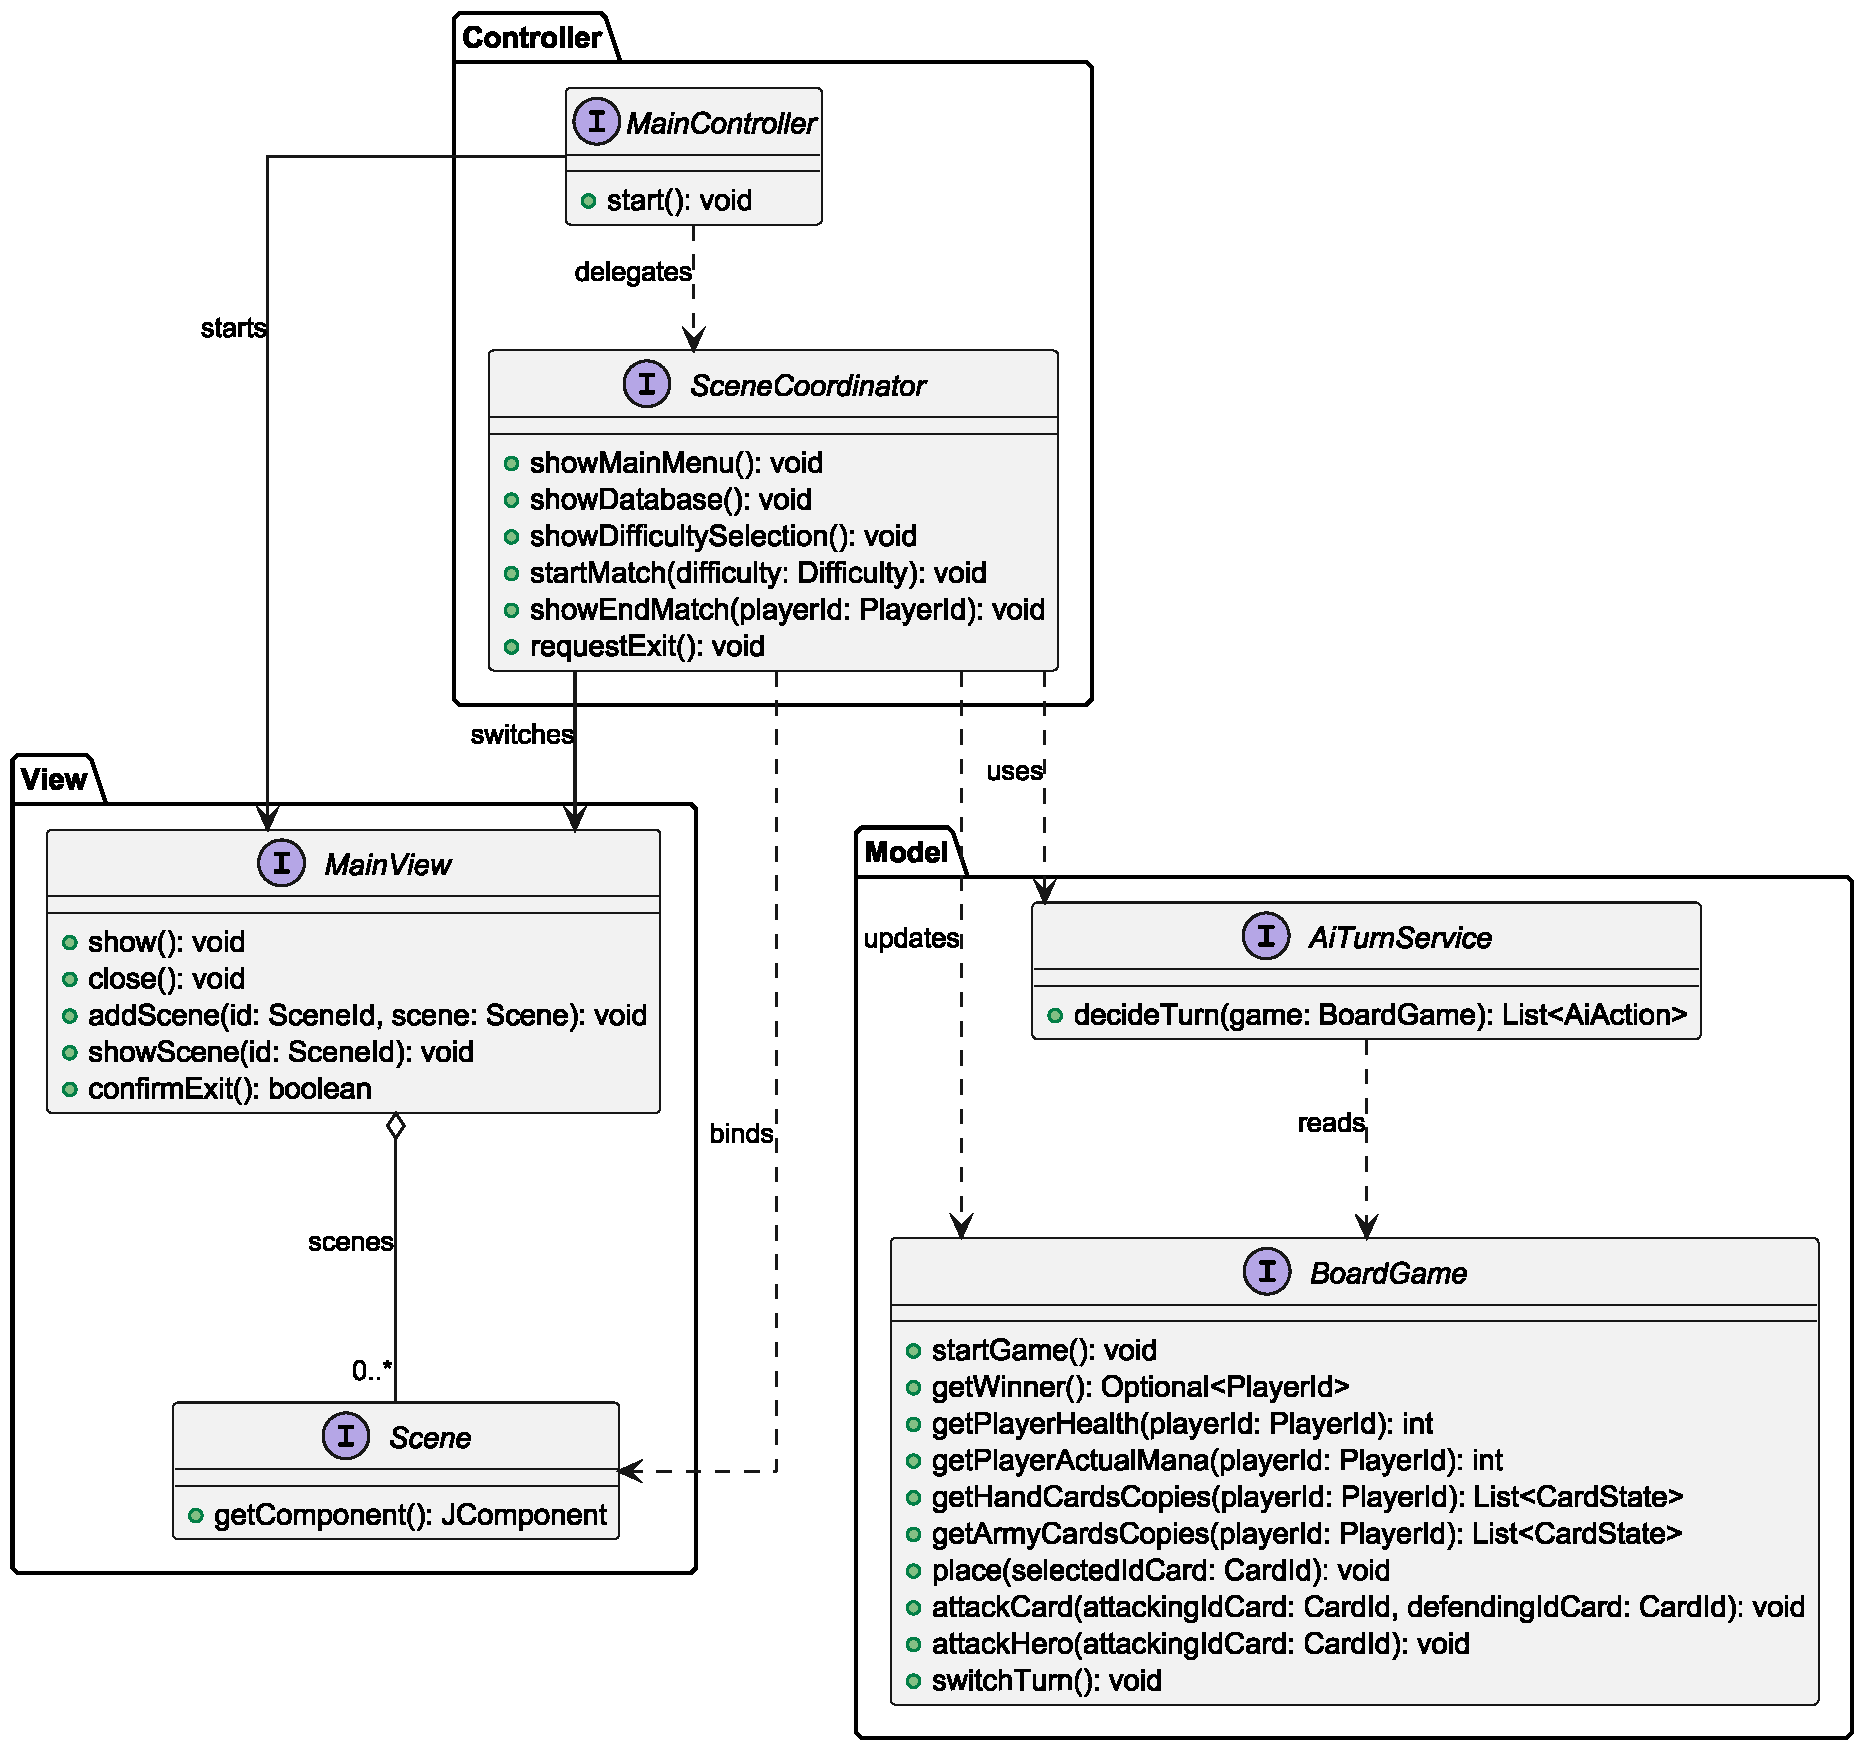
\includegraphics[width=\textwidth]{UMLs/ArchitetturaMVC.pdf}
    \caption{Schema UML dell'architettura MVC dell'applicazione.}
\end{figure}

\section{Design Dettagliato}

\subsection{Simone Marsili}

\subsubsection{Gestione delle carte di gioco}

\textbf{Problema:} Le carte nel gioco possono essere di varie tipologie, come
\texttt{Creatures} e \texttt{Spells} (requisito opzionale del progetto), e il
sistema deve essere estendibile a nuove aggiunte e tipi di carte. Inoltre le
carte devono contenere un apposito identificatore, il quale permette le
operazioni sul modello durante la partita e impedisce la duplicazione di dati
tra istanze. Tuttavia è necessario separare l'identità runtime delle carte
dalla loro definizione statica. Si è cercato inoltre un modo per separare
efficacemente dichiarazioni e implementazioni delle creature.

\textbf{\\Soluzione:} L'interfaccia \texttt{Creature} rappresenta una tipologia
di carte schierabili, e l'implementazione \texttt{CreatureImpl} si compone di
un \texttt{CardId}, il quale informa sulla tipologia di carta e sulla sua
numerazione univoca nel game, e di una \texttt{CreatureDefinition}, che
rappresenta invece l'aspetto statico della carta (le sue statistiche base).
L'implementazione delle creature è stata realizzata tramite una
\textit{Simple Factory}, che rende il codice facilmente estendibile e
manutenibile. La factory utilizza un \texttt{IdGenerator}, che non istanzia
autonomamente, ma che riceve tramite costruttore, riducendo l'accoppiamento e
migliorando testabilità ed estendibilità.

\begin{figure}[htbp]
    \centering
    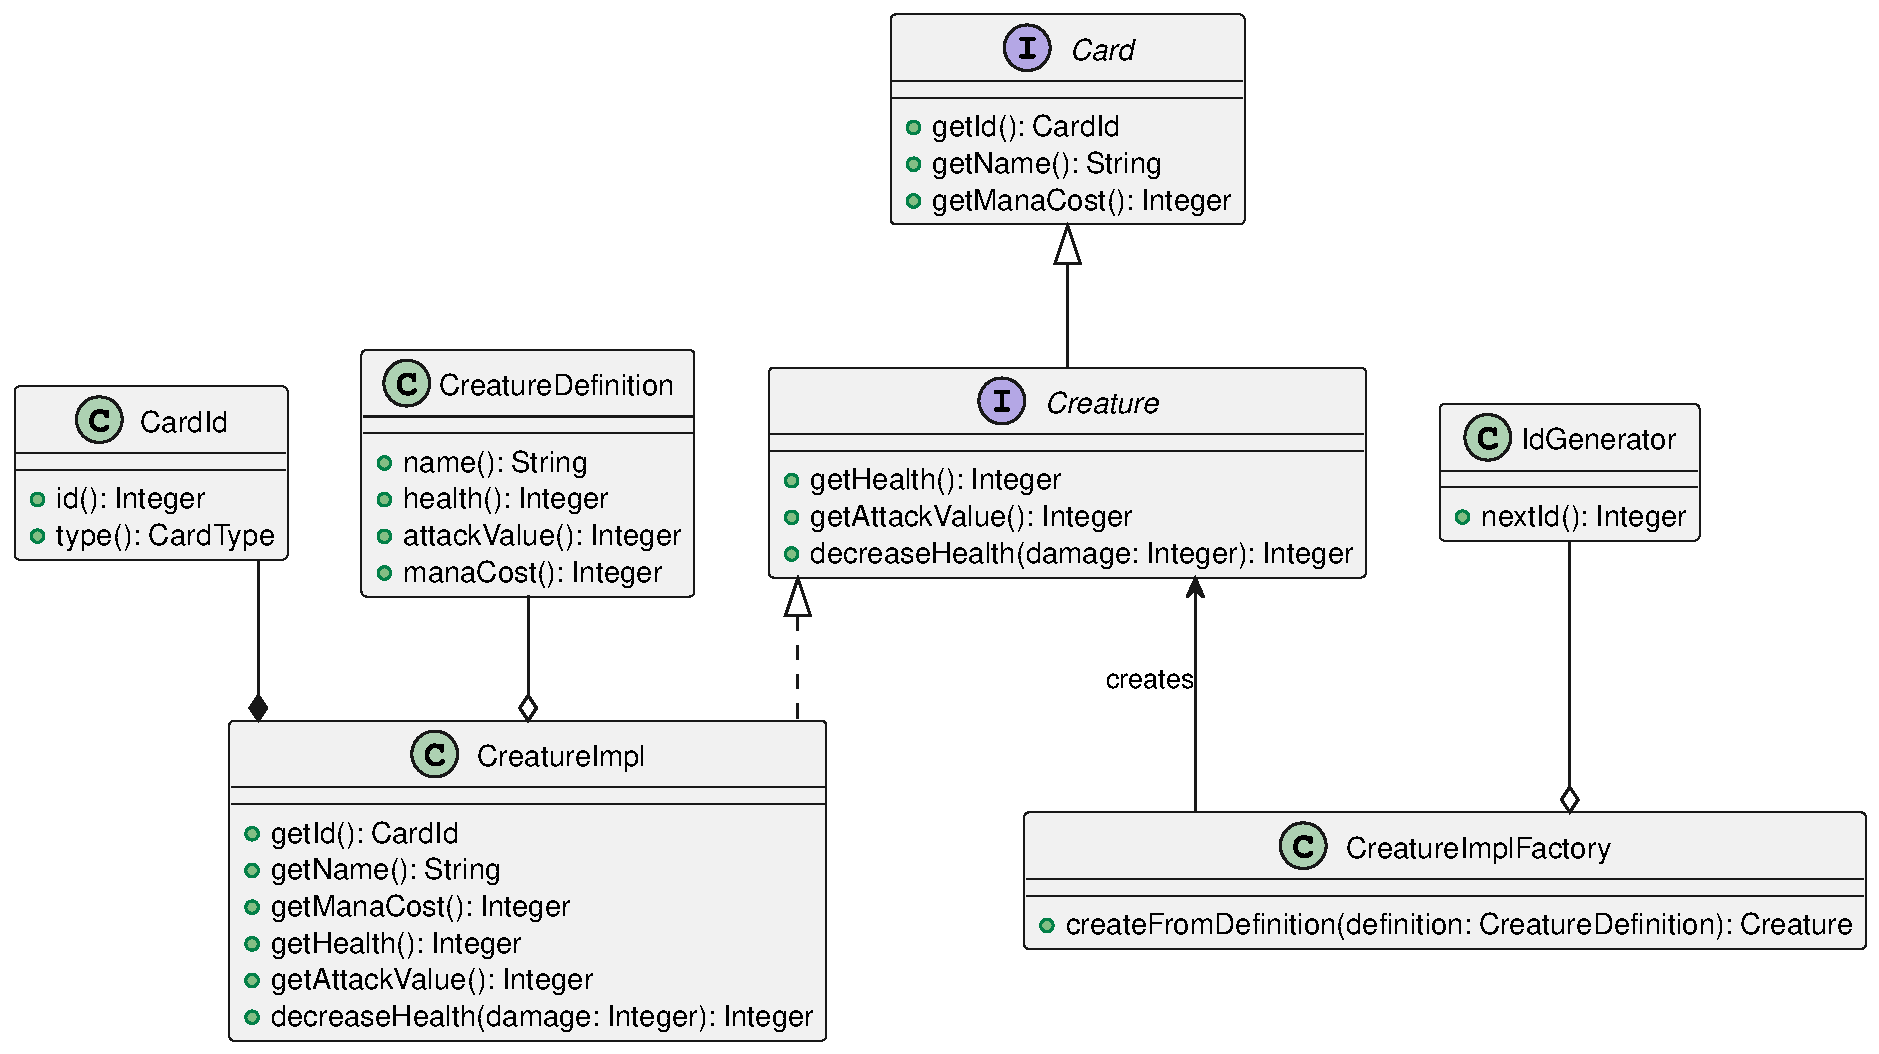
\includegraphics[width=\textwidth]{UMLs/Card.pdf}
    \caption{Schema UML della gestione delle carte e delle relative definizioni.}
\end{figure}

\subsubsection{Gestione del database di carte}

\textbf{Problema:} Il gioco prevede la presenza di un database contenente tutte
le carte che possono comparire in un match. Il sistema necessita di una
rappresentazione centralizzata e facilmente estendibile delle carte, caricata
da una fonte esterna (file), mantenendo separata la logica di parsing dalla
logica di dominio. Inoltre, il database deve gestire esclusivamente dati
statici delle carte, risultando indipendente dall'identità runtime delle
istanze generate durante la partita.

\textbf{\\Soluzione:} Il database gestisce esclusivamente definizioni statiche
delle carte (\texttt{CreatureDefinition}), risultando completamente
disaccoppiato dal concetto di identità runtime, che viene invece introdotto
solo in fase di creazione delle istanze.

Inoltre la creazione di un'istanza del database avviene tramite apposita
Factory statica, che utilizza componenti distinti per la lettura del file e per
il parsing del contenuto, mantenendo separate le responsabilità di accesso ai
dati e interpretazione degli stessi.

Le interfacce \texttt{Parser\textless{}T\textgreater{}} e
\texttt{FullReader\textless{}T\textgreater{}} rappresentano due strategie
intercambiabili (pattern \textit{Strategy}) rispettivamente per
l'interpretazione dei dati e per la lettura delle sorgenti, permettendo di
estendere facilmente il sistema a nuovi formati o fonti dati.

\begin{figure}[htbp]
    \centering
    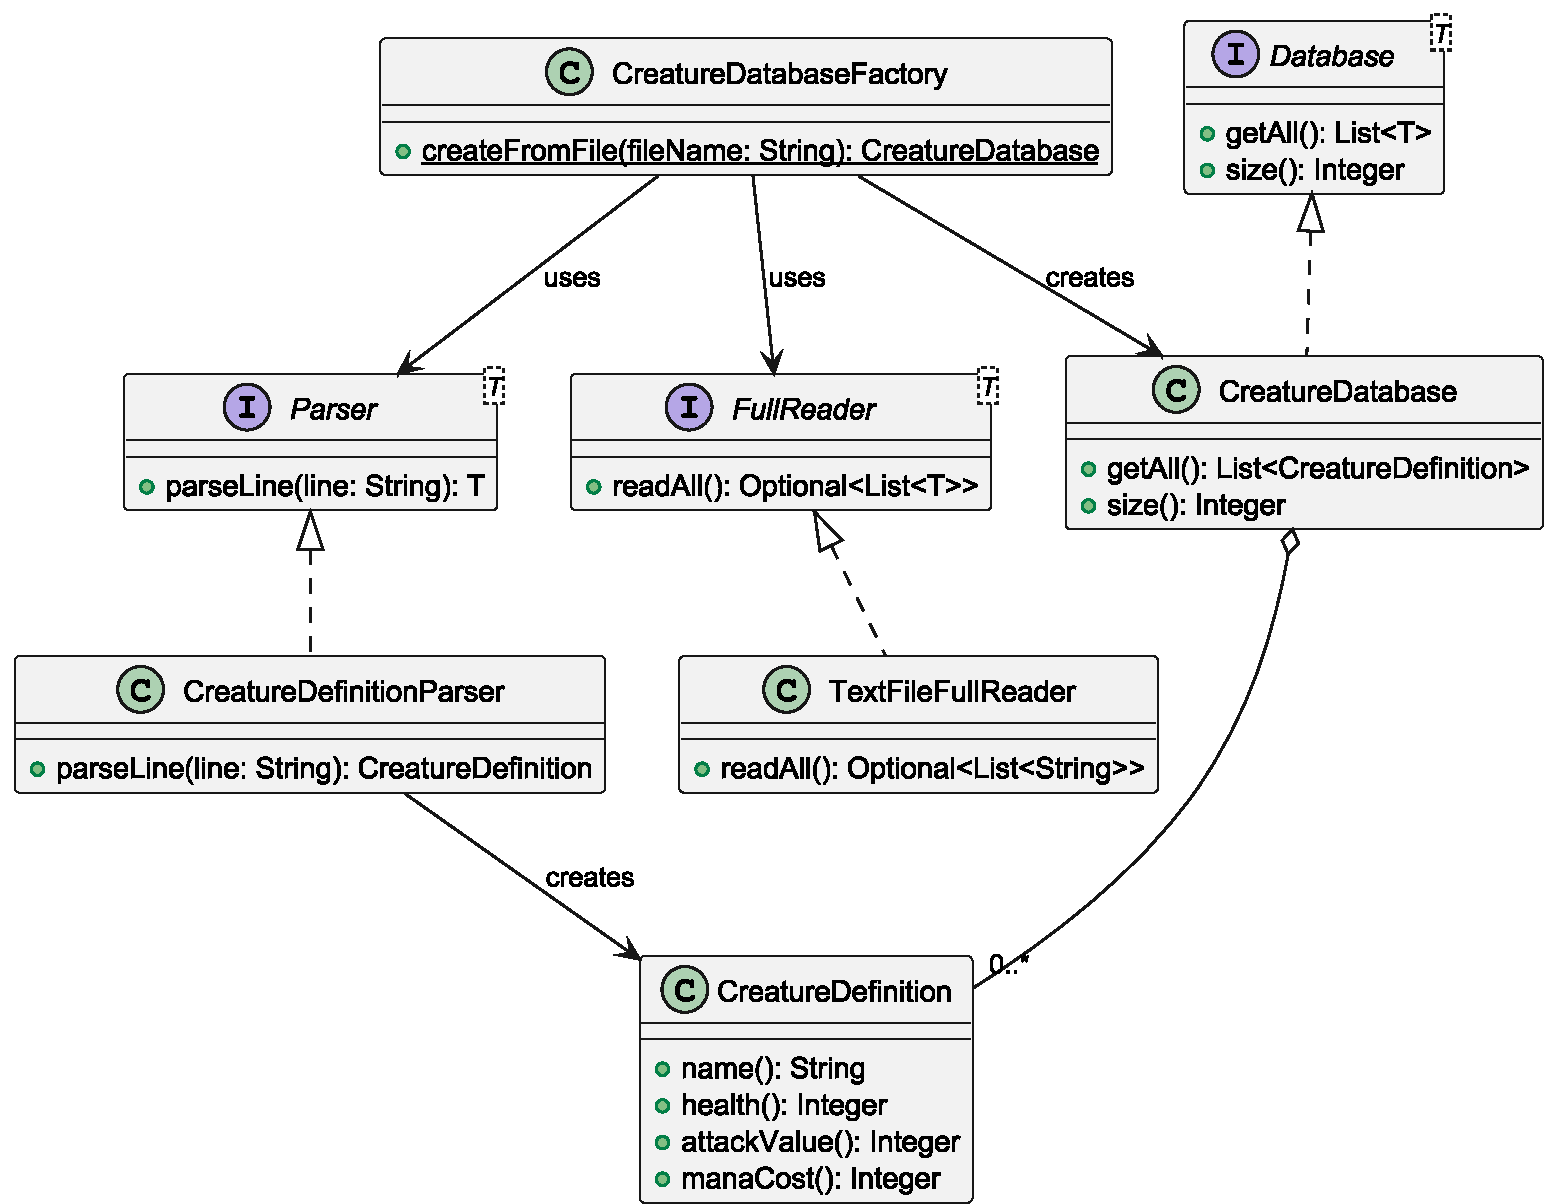
\includegraphics[width=\textwidth]{UMLs/Database.pdf}
    \caption{Schema UML del database delle carte e dei componenti di lettura e parsing.}
\end{figure}

\subsubsection{Gestione del deck}

\textbf{Problema:} Il gioco richiede la creazione di un mazzo da cui il
giocatore possa pescare progressivamente le carte durante la partita. Tuttavia,
il mazzo non deve essere costruito manualmente né contenere direttamente le
definizioni statiche presenti nel database: ogni carta inserita nel deck deve
essere una nuova istanza runtime, dotata del proprio identificatore.

Un ulteriore problema riguarda la composizione del mazzo. Non tutte le carte
dovrebbero avere necessariamente la stessa probabilità di comparire: ad esempio,
carte più forti possono essere rese meno frequenti rispetto a carte più deboli,
così da ottenere un deck più bilanciato. Il sistema deve quindi permettere di
modificare il criterio di selezione delle carte senza intervenire sulla logica
interna del mazzo o sulla factory che lo costruisce.

\textbf{\\Soluzione:} La gestione del mazzo è stata separata dalla sua
costruzione. L'interfaccia \texttt{Deck} espone soltanto le operazioni
necessarie durante la partita, cioè la pesca di una carta tramite
\texttt{draw()} e la consultazione del numero di carte rimanenti tramite
\texttt{getRemaining()}. L'implementazione \texttt{DeckImpl} incapsula quindi
la lista delle carte effettivamente presenti nel mazzo e si occupa solo della
loro gestione runtime.

La creazione del mazzo è invece affidata a \texttt{DeckFactory}. Questa classe
riceve tramite costruttore un \texttt{CreatureDatabase}, da cui ottiene le
definizioni statiche delle creature, e una \texttt{CreatureImplFactory}, usata
per trasformare ogni \texttt{CreatureDefinition} selezionata in una vera
istanza runtime di \texttt{Card}. In questo modo il database resta separato
dall'identità delle carte usate nella partita, che viene introdotta solo al
momento della generazione del deck.

La classe \texttt{DeckFactory} realizza sostanzialmente una
\textit{Simple Factory}, poiché centralizza la logica di creazione del mazzo e
nasconde al resto del modello i dettagli necessari alla sua costruzione
(recupero definizioni dal database, creazione istanze runtime, selezione
pesata, mescolamento finale\ldots{}).

Il metodo \texttt{createWeighted(size, strategy)} costruisce un mazzo della
dimensione richiesta usando una \texttt{WeightStrategy}. In questa versione
implementata, la factory calcola il peso associato a ciascuna definizione e usa
tale valore per effettuare una selezione casuale non uniforme. In seguito le
carte generate vengono mescolate prima della creazione del \texttt{DeckImpl},
così da evitare che l'ordine del database influenzi l'ordine di pesca.

Nel caso in cui la dimensione richiesta sia maggiore o uguale al numero di
carte presenti nel database, la factory inserisce almeno una copia di ogni
creatura disponibile e completa poi il mazzo tramite selezione pesata. Questo
evita che, in mazzi abbastanza grandi, alcune creature non compaiano mai solo
per effetto della casualità. Quando invece la dimensione richiesta è inferiore
al numero di definizioni disponibili, l'intero mazzo viene generato tramite
selezione pesata.

La soluzione usa il pattern \textit{Strategy} attraverso l'interfaccia
{\texttt{WeightStra\-tegy}}. Tale interfaccia rappresenta l'algoritmo
intercambiabile con cui viene calcolata l'importanza di una
\texttt{CreatureDefinition} durante la costruzione del mazzo.
\texttt{DeckFactory} usa la strategia senza conoscere il criterio concreto
adottato, rendendo possibile introdurre in futuro nuove politiche di
generazione del deck senza modificare la factory. Inoltre la
\texttt{WeightStrategy} è una functional interface, il che rende molto facile
creare al volo delle nuove strategie.

\begin{figure}[htbp]
    \centering
    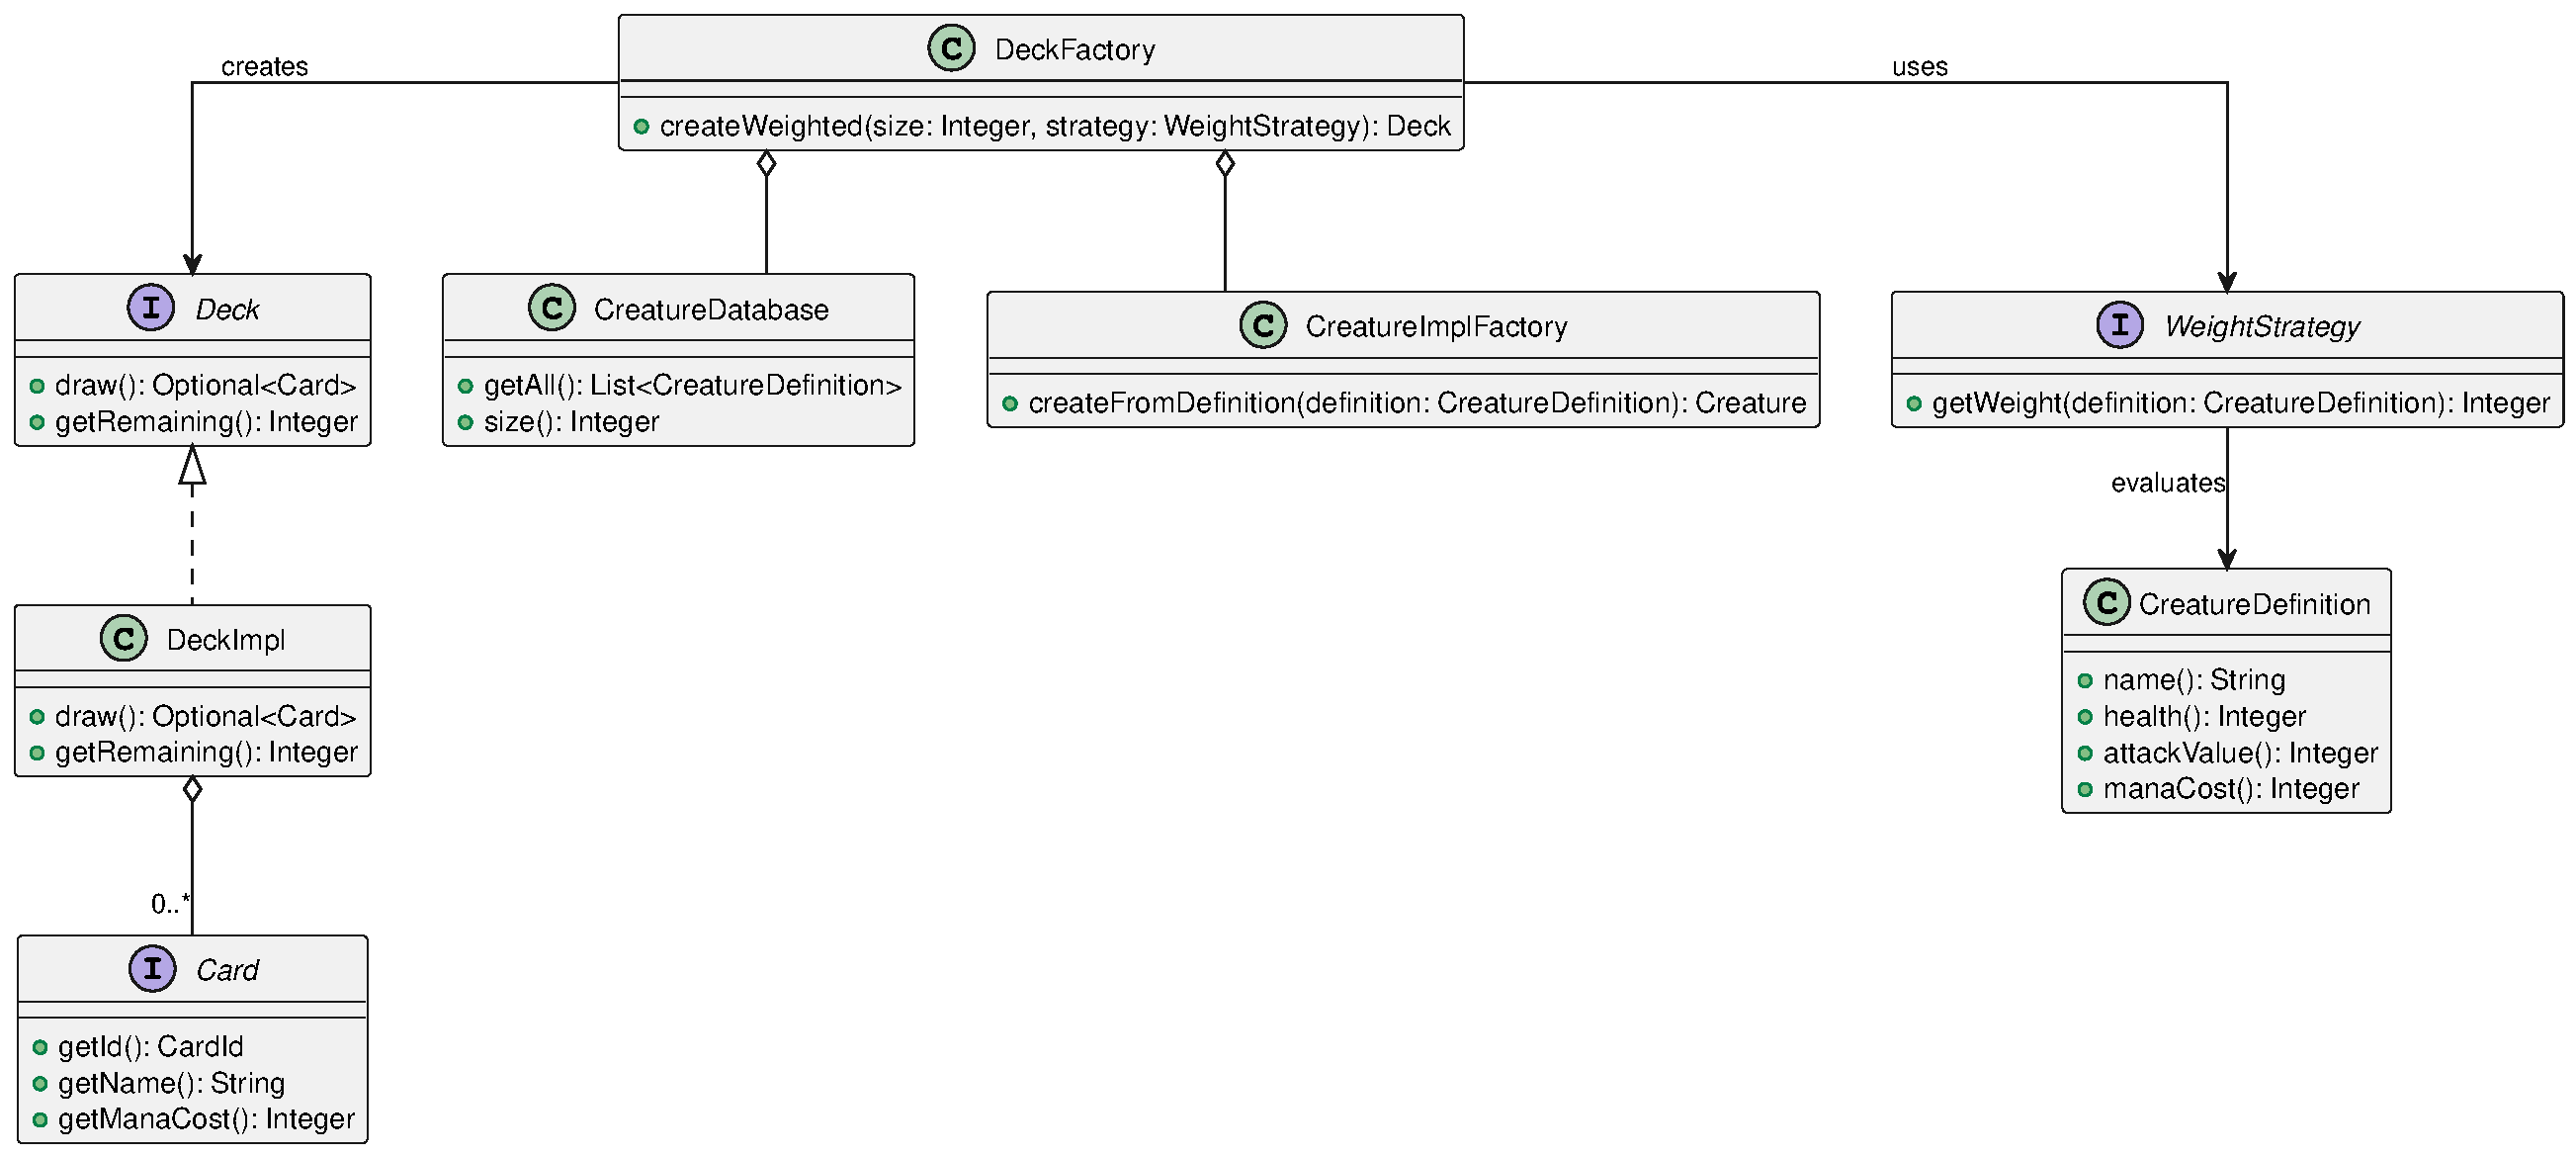
\includegraphics[width=\textwidth]{UMLs/Deck.pdf}
    \caption{Schema UML della costruzione e gestione del mazzo di gioco.}
\end{figure}

\subsubsection{Gestione dell'aggiornamento della view}

\textbf{Problema:} Durante lo svolgimento di una partita, lo stato del modello
cambia frequentemente: la partita viene avviata, il turno passa da un giocatore
all'altro, vengono pescate o giocate carte, cambiano i punti vita di creature e
giocatori, varia il mana disponibile e alcune carte possono essere distrutte o
bruciate. Tutti questi cambiamenti devono essere riflessi nella schermata di
gioco in modo coerente e tempestivo.

Una prima soluzione possibile sarebbe stata lasciare al controller il compito di
aggiornare manualmente la view dopo ogni operazione eseguita sul modello. Questa
scelta, però, avrebbe reso il controller responsabile anche dei dettagli di
aggiornamento grafico, aumentando il suo accoppiamento sia con il model sia con
la view.

Un'altra alternativa sarebbe stata usare una notifica generica, basata su un
unico metodo come \texttt{update()}. In questo caso, però, la view avrebbe
ricevuto solo l'informazione che qualcosa nel modello è cambiato, dovendo poi
interrogare il model per ricostruire lo stato aggiornato. Questa variante è
stata scartata perché avrebbe richiesto alla view di conoscere più dettagli del
modello e avrebbe reso meno esplicito il significato dei singoli aggiornamenti.

Il problema era quindi progettare un meccanismo che permettesse al model di
comunicare alla view gli eventi rilevanti della partita, fornendo direttamente
le informazioni necessarie all'aggiornamento grafico, senza costringere la view
a richiedere ogni volta lo stato aggiornato.

\textbf{\\Soluzione:} La soluzione adottata applica il pattern
\textit{Observer} in una variante di tipo \textit{push model}. Il modello della
partita è l'oggetto osservabile, mentre la view della partita è uno degli
osservatori registrati. Quando lo stato del model cambia, il model non invia
una notifica generica, ma comunica direttamente quale evento è avvenuto e quali
dati aggiornati sono necessari per gestirlo.

L'interfaccia \texttt{ObservableGame} definisce il contratto degli oggetti
osservabili, esponendo i metodi per registrare e rimuovere osservatori.

L'interfaccia \texttt{BoardGame} estende \texttt{ObservableGame}, rendendo
esplicito che il modello principale della partita può essere osservato. La
classe {\texttt{BoardGame\-Impl}} implementa questo contratto, mantiene gli
observer registrati e li notifica opportunamente quando si verifica un
cambiamento significativo nello stato della partita.

Gli observer sono rappresentati dall'interfaccia \texttt{GameObserver}. A
differenza di una versione minimale del pattern \textit{Observer}, non è stato
usato un unico metodo generico di aggiornamento. L'interfaccia espone invece
più metodi specifici, ciascuno associato a un evento rilevante del gioco.

Questa scelta rende la comunicazione tra model e view più esplicita. Il nome
del metodo identifica l'evento avvenuto, mentre i parametri trasportano già le
informazioni aggiornate.

Sul lato view, \texttt{MatchView} estende \texttt{GameObserver}. In questo
modo, una schermata di partita è anche un osservatore del modello. La classe
concreta \texttt{MatchScene} implementa \texttt{MatchView} e definisce come
tradurre ciascun evento ricevuto in un aggiornamento grafico.

Il collegamento tra model e view viene effettuato dal controller, che registra
la view come observer del model. Il model, però, non conosce la classe concreta
\texttt{MatchScene}: conosce solo l'interfaccia \texttt{GameObserver}. Questo
mantiene basso l'accoppiamento tra le componenti e rispetta la separazione
prevista dall'architettura MVC.

La soluzione ha anche un compromesso: l'interfaccia \texttt{GameObserver} cresce
all'aumentare degli eventi osservabili. Se in futuro venissero introdotti nuovi
eventi di gioco, potrebbe essere necessario aggiungere nuovi metodi
all'interfaccia e aggiornare le classi che la implementano. Nel contesto del
progetto, però, questo costo è accettabile, perché gli eventi rilevanti della
partita sono limitati e ben definiti. In cambio, si ottiene una comunicazione
più leggibile, più controllata e più aderente al dominio del gioco.

\begin{figure}[htbp]
    \centering
    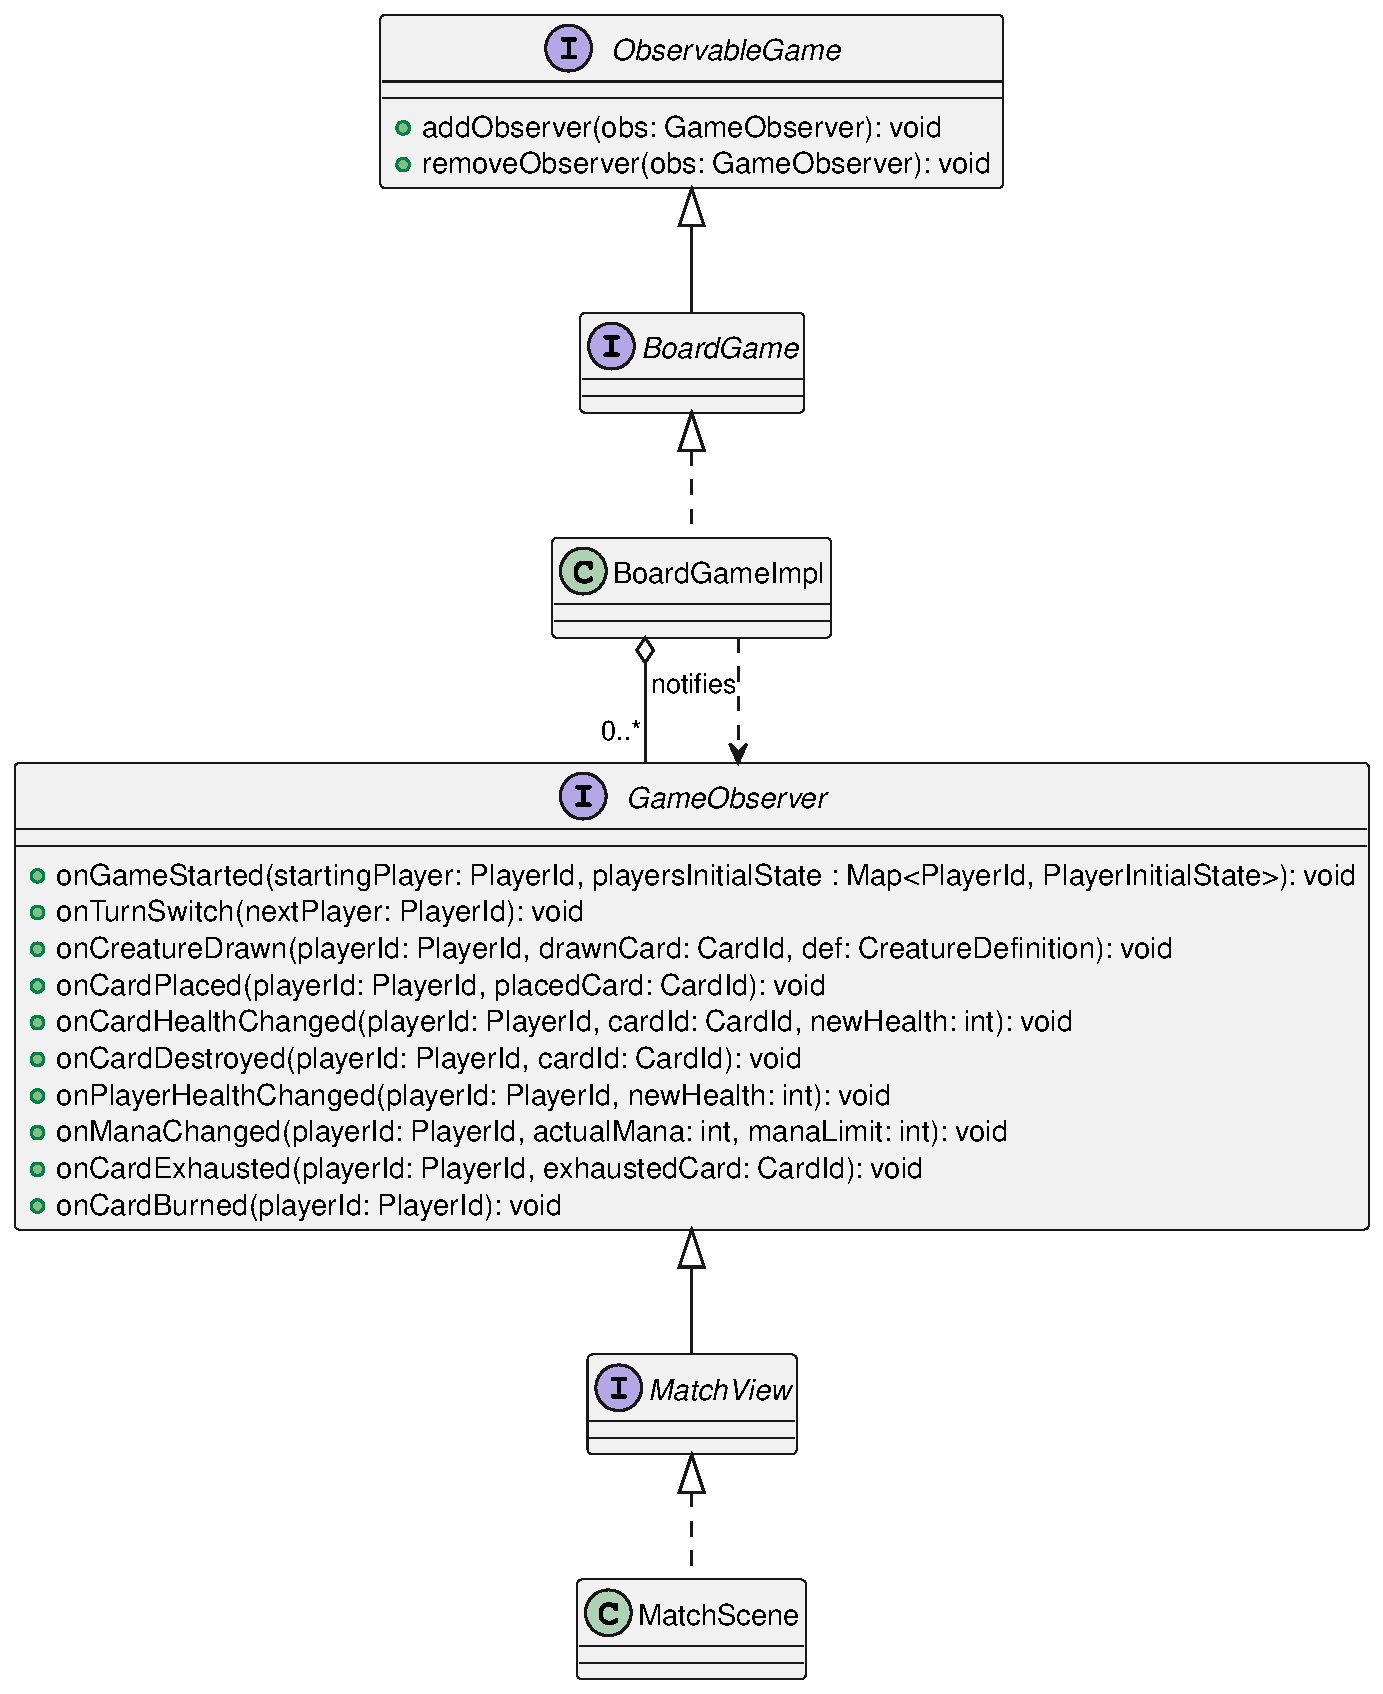
\includegraphics[width=\textwidth]{UMLs/Observer.pdf}
    \caption{Schema UML del meccanismo di aggiornamento della view tramite observer.}
\end{figure}

\newpage

\subsection{Francesco Dama}

\subsubsection{Problema 1:Gestione della mano del giocatore}

Nel gioco ogni giocatore deve poter gestire una mano di carte pescate dal deck durante la partita. 
La mano rappresenta una struttura centrale del gameplay, poiché viene continuamente modificata: nuove carte vengono aggiunte
 tramite pesca, alcune vengono rimosse quando giocate, e il numero massimo di carte deve essere limitato.
Una possibile soluzione sarebbe stata trattare la mano semplicemente come una lista esposta 
direttamente dal giocatore, lasciando al resto del sistema la responsabilità di controllarne dimensione, inserimenti e rimozioni.
Questa scelta, però, avrebbe distribuito la logica della mano in più punti del codice, 
aumentando l'accoppiamento e rendendo più difficile garantire la coerenza dello stato.
Il problema era quindi progettare una componente autonoma che incapsulasse completamente la gestione
della mano, mantenendo separate le responsabilità del giocatore da quelle della collezione di carte possedute.

\textbf{\\Soluzione:}
La soluzione adottata introduce l’interfaccia \texttt{Hand}, che rappresenta il contratto
astratto di una mano di gioco. Essa espone soltanto le operazioni rilevanti per il dominio,
come l’aggiunta, la rimozione e la consultazione delle carte presenti.

La classe \texttt{HandImpl} implementa tale comportamento incapsulando internamente la struttura
dati concreta utilizzata per memorizzare le carte. In questo modo il resto del modello non dipende 
direttamente dalla rappresentazione interna della mano.
La responsabilità del giocatore (\texttt{PlayerImpl}) viene così semplificata: il giocatore possiede una mano,
ma non gestisce direttamente la logica di manipolazione delle carte al suo interno. 
Questo migliora la separazione delle responsabilità e mantiene il modello più modulare.
La soluzione applica inoltre il principio di \textit{information hiding}: il resto del sistema 
interagisce con la mano esclusivamente tramite l'interfaccia \texttt{Hand}, senza conoscere dettagli implementativi.

%\begin{figure}[htbp]
%\centering
%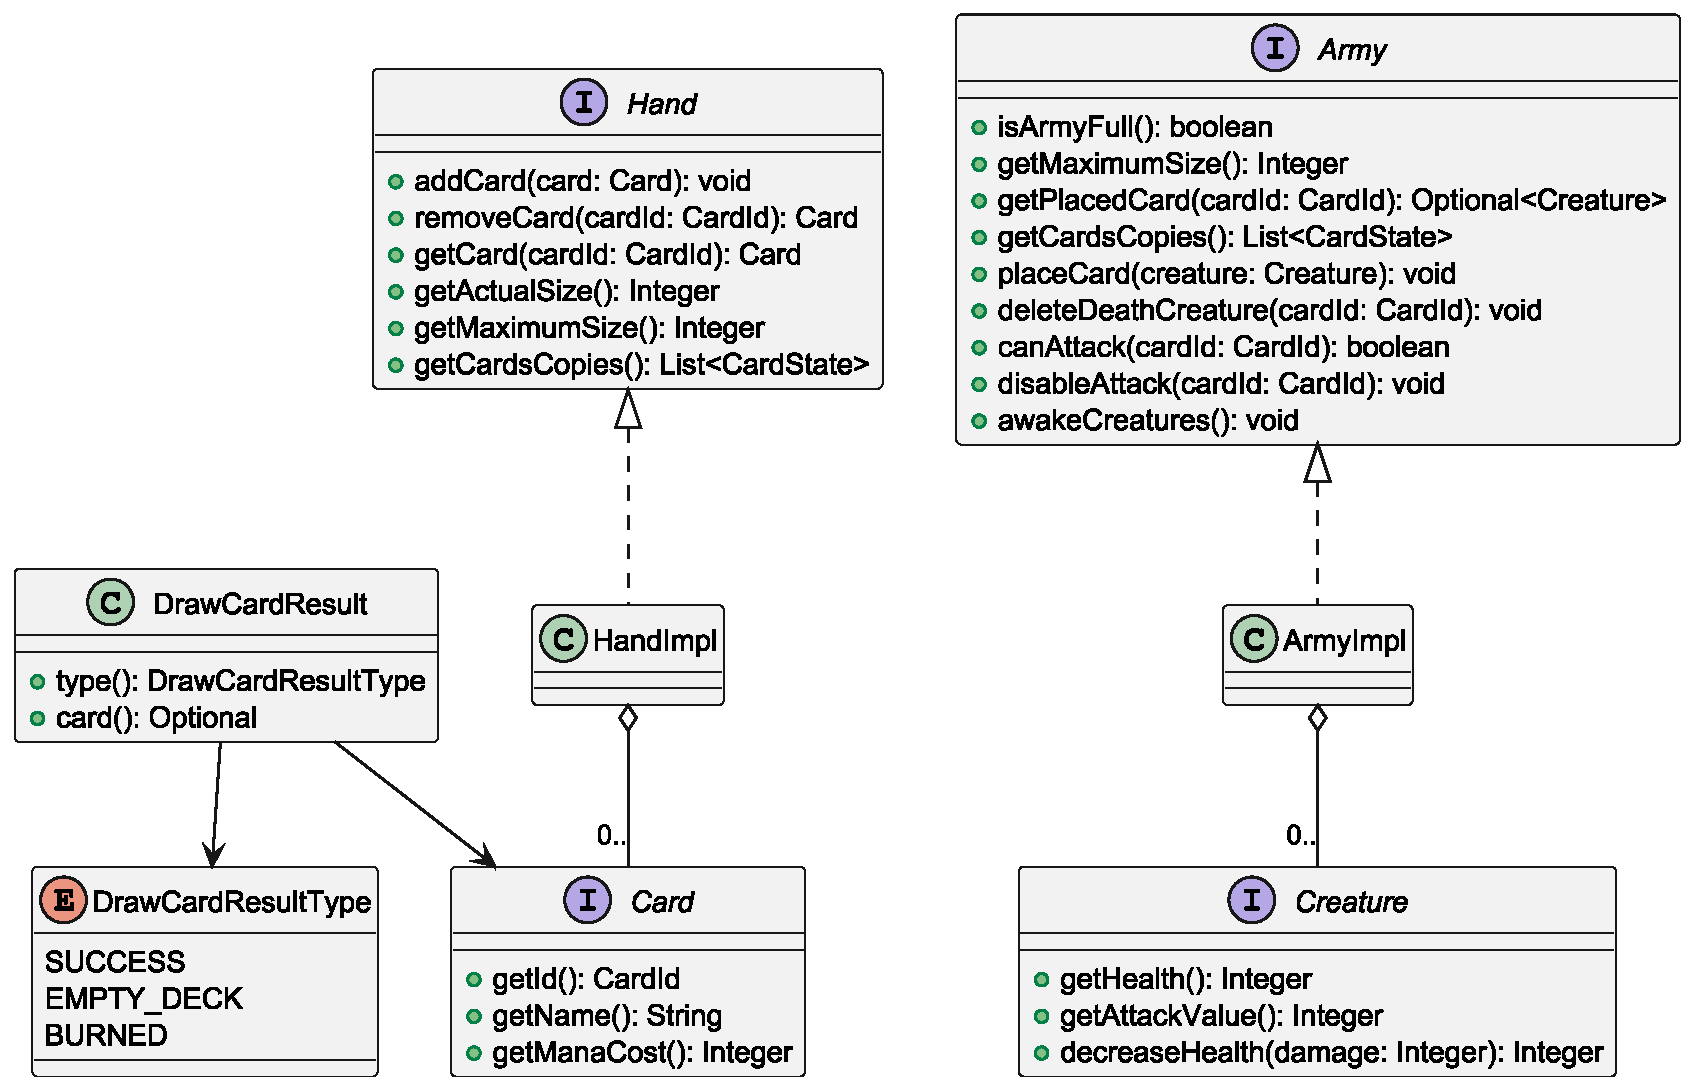
\includegraphics[width=0.85\textwidth]{UMLs/PoliticaPescaggioMano.pdf}
%\caption{Schema UML della gestione della mano del giocatore.}
%\end{figure}

\subsubsection{Problema 2:Gestione della pesca delle carte e degli esiti della pesca}

Durante la partita un giocatore può pescare carte dal proprio deck.
Tuttavia l'operazione di pesca non produce sempre lo stesso risultato: il deck potrebbe essere vuoto,
oppure la mano potrebbe essere piena e la carta pescata dovrebbe quindi essere bruciata.

Una possibile soluzione sarebbe stata usare valori speciali (\texttt{null})
oppure lanciare eccezioni per rappresentare i casi particolari della pesca. 
Questa alternativa è stata scartata perché avrebbe reso meno esplicita la semantica 
dell'operazione e avrebbe distribuito la gestione dei casi speciali nel controller o nel model.

Il problema era quindi rappresentare in modo chiaro e tipizzato tutti i possibili esiti dell'operazione
di pesca, mantenendo il codice leggibile ed evitando ambiguità.

\textbf{\\Soluzione:}
La soluzione adottata introduce il tipo \texttt{DrawCardResult}, che rappresenta esplicitamente
il risultato di una pesca. Tale oggetto contiene tutte le informazioni necessarie per descrivere l'esito dell'operazione.

Il tipo di risultato viene modellato tramite l'enumerazione 
\texttt{DrawCardResultType}, che distingue i vari scenari possibili, come:
\begin{itemize}
\item pesca completata correttamente;
\item deck vuoto;
\item carta bruciata per mano piena.
\end{itemize}

In questo modo il modello comunica chiaramente cosa è accaduto senza ricorrere a valori speciali o controlli impliciti.

La soluzione segue un approccio simile al pattern \textit{Result Object}:
invece di restituire semplicemente una carta o fallire tramite eccezioni,
il metodo restituisce un oggetto che rappresenta semanticamente l'esito dell'operazione.

Questo rende il codice più robusto e leggibile, perché i casi gestibili dal dominio
vengono esplicitati direttamente nel tipo restituito.

%\begin{figure}[htbp]
%\centering
%\includegraphics[width=0.7\textwidth]{UMLs/DrawCardResult.pdf}
%\caption{Schema UML della gestione degli esiti della pesca.}
%\end{figure}

\subsubsection{Problema 3:Gestione dello stato del giocatore}

Nel gioco il giocatore rappresenta una componente complessa del modello. Ogni giocatore possiede:
\begin{itemize}
\item un deck;
\item una mano;
\item un esercito di creature schierate;
\item punti vita;
\item mana disponibile;
\item un'identità logica all'interno della partita.
\end{itemize}

Una possibile soluzione sarebbe stata concentrare tutta questa logica direttamente all'interno
della classe del giocatore, rendendola responsabile sia della gestione delle risorse sia della
logica di combattimento e del turno. Questa scelta, però, avrebbe prodotto una classe molto accoppiata e difficile da estendere.

Il problema era quindi modellare il giocatore come aggregatore delle varie componenti del gameplay,
delegando però le responsabilità specifiche a classi dedicate.

\textbf{\\Soluzione:}
La soluzione adottata utilizza l'interfaccia \texttt{Player} come rappresentazione astratta di un giocatore della partita.

La classe \texttt{PlayerImpl} coordina le varie componenti che costituiscono lo stato del giocatore:
\begin{itemize}
\item \texttt{Hand} per la gestione delle carte in mano;
\item \texttt{Army} per le creature schierate;
\item \texttt{Deck} per la pesca;
\item \texttt{ManaManager} per la gestione del mana.
\end{itemize}

Questa scelta permette di suddividere il comportamento in componenti specializzate,
mantenendo il giocatore come coordinatore logico dello stato.
L'identità del giocatore viene separata tramite \texttt{PlayerId}, mentre \texttt{PlayerType}
rappresenta la natura del giocatore (umano o IA). In questo modo il sistema può distinguere chiaramente
il ruolo del giocatore senza introdurre controlli sparsi nel codice.
La creazione dei giocatori viene inoltre centralizzata tramite \texttt{PlayerFactory},
che costruisce correttamente tutte le dipendenze necessarie. Questa soluzione riduce l'accoppiamento e nasconde 
la complessità di inizializzazione al resto del sistema.

La gestione del mana viene delegata a \texttt{ManaManager}, evitando che \texttt{PlayerImpl}
debba conoscere i dettagli delle regole di incremento e consumo del mana durante i turni.

La soluzione applica quindi una combinazione di:
\begin{itemize}
\item composizione;
\item separation of concerns;
\item factory pattern.
\end{itemize}

%\begin{figure}[htbp]
%\centering
%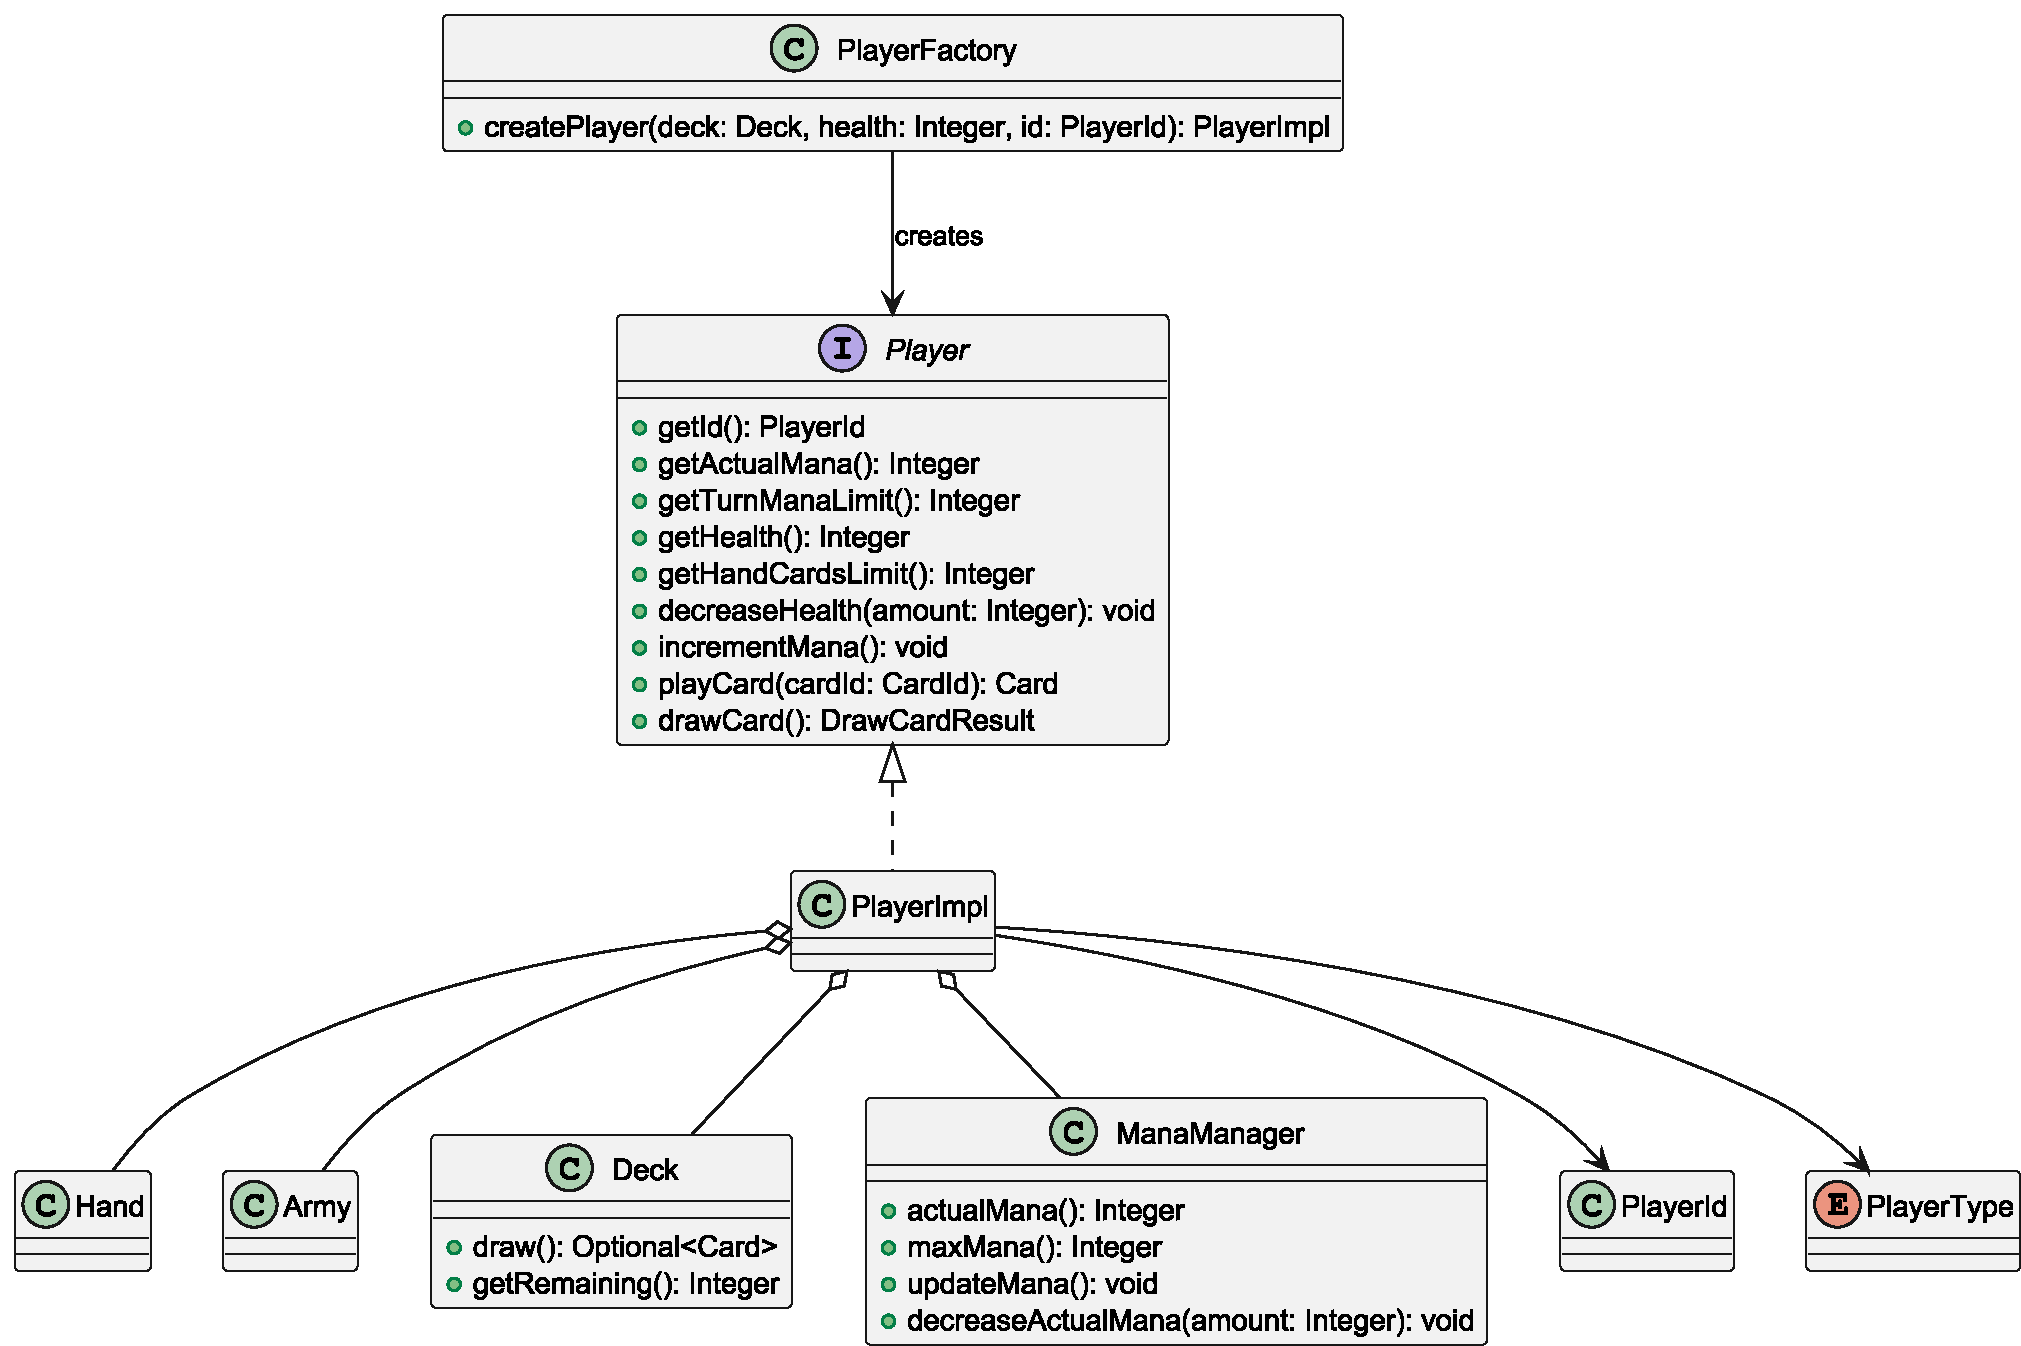
\includegraphics[width=0.95\textwidth]{UMLs/GestioneStatoGiocatore.pdf}
%\caption{Schema UML della gestione dello stato del giocatore.}
%\end{figure}

\subsubsection{Problema 1:Gestione delle creature schierate sul campo}

Durante la partita ogni giocatore può schierare creature sul campo di gioco. Tali creature devono essere
gestite separatamente dalla mano e dal deck, poiché rappresentano lo stato attivo del combattimento.

Una possibile soluzione sarebbe stata trattare le creature schierate come una semplice lista interna al giocatore.
Tuttavia questa scelta avrebbe accoppiato fortemente la logica del combattimento con quella del giocatore stesso.

Il problema era quindi creare una struttura dedicata alla gestione delle creature presenti sul board, 
mantenendo separate le responsabilità del giocatore dalla gestione delle unità schierate.

\textbf{\\Soluzione:}
La soluzione adottata introduce l'interfaccia \texttt{Army},
che rappresenta l'insieme delle creature schierate da un giocatore.

L'implementazione \texttt{ArmyImpl} incapsula completamente la gestione delle creature
presenti sul campo, occupandosi delle operazioni di inserimento, rimozione e consultazione.

Il giocatore possiede quindi un'istanza di \texttt{Army}, ma non gestisce direttamente
la struttura interna delle creature schierate.

Questa soluzione migliora la modularità del sistema e rende più semplice estendere in futuro
le regole legate al campo di gioco, ad esempio:
\begin{itemize}
\item limiti sul numero di creature;
\item ordinamento sul board;
\item effetti ad area;
\item gestione di evocazioni speciali.
\end{itemize}

La soluzione segue il principio di composizione, mantenendo il board del giocatore come componente autonoma del modello.

%\begin{figure}[htbp]
%\centering
%\includegraphics[width=0.8\textwidth]{UMLs/ArmyManagement.pdf}
%\caption{Schema UML della gestione delle creature schierate.}
%\end{figure}

\subsubsection{Problema 3:Gestione del turno e delle risorse di mana}

Il sistema di turni rappresenta una parte critica della logica di gioco. A ogni cambio turno devono essere aggiornati:
\begin{itemize}
\item il giocatore attivo;
\item il mana disponibile;
\item lo stato di esaurimento delle creature;
\item eventuali operazioni automatiche di inizio turno.
\end{itemize}

Una possibile soluzione sarebbe stata implementare tutta questa logica direttamente all'interno
di \texttt{BoardGameImpl}, centralizzando l'intero flusso della partita in un'unica classe.
Questa scelta, però, avrebbe prodotto una classe troppo grande e difficile da mantenere.

Il problema era quindi isolare la logica specifica di gestione dei turni,
mantenendola separata dalla restante logica del board game.

\textbf{\\Soluzione:}
La soluzione adottata introduce il componente \texttt{TurnManager}, definito internamente a \texttt{BoardGameImpl}, responsabile esclusivamente della gestione dell’alternanza dei turni.

\texttt{TurnManager} coordina:
\begin{itemize}
\item il passaggio del turno tra i giocatori;
\item l'aggiornamento del mana;
\item il reset dello stato delle creature;
\item le operazioni automatiche di inizio turno.
\end{itemize}

La gestione del mana viene ulteriormente delegata a \texttt{ManaManager},
che incapsula le regole di incremento e consumo delle risorse.

Questa separazione permette di mantenere \texttt{BoardGameImpl} focalizzata sulla coordinazione generale
della partita, evitando che conosca tutti i dettagli operativi del turno.

La soluzione migliora:
\begin{itemize}
\item leggibilità;
\item manutenibilità;
\item separazione delle responsabilità.
\end{itemize}

Inoltre rende più semplice modificare in futuro le regole del turno senza impattare il resto del modello.

%\begin{figure}[htbp]
%\centering
%\includegraphics[width=0.7\textwidth]{UMLs/GestioneTurnoRIsorse.pdf.pdf}
%\caption{Schema UML della gestione dei turni e del mana.}
%\end{figure}

\subsection{Lorenzo Mercuriali}

\subsubsection{Problema 1}

\textbf{Problema:}

\textbf{\\Soluzione:}

\subsubsection{Problema 2}

\textbf{Problema:}

\textbf{\\Soluzione:}

\subsubsection{Problema 3}

\textbf{Problema:}

\textbf{\\Soluzione:}

\subsubsection{Problema 4}

\textbf{Problema:}

\textbf{\\Soluzione:}

\subsection{Massimiliano Ria}

\subsubsection{Adattamento dell'interfaccia a diverse risoluzioni}

\textbf{Problema:} Dopo aver ottenuto un'interfaccia grafica funzionante e
un'architettura coerente, è emersa la necessità di mantenerne l'aspetto
uniforme su risoluzioni e rapporti d'aspetto diversi.

\textbf{\\Soluzione:} Un primo approccio al problema è stato l'introduzione della
classe \texttt{ViewMetrics}, usata come punto di accesso unico alle principali
dimensioni grafiche dell'applicazione. Nella sua versione iniziale, tali misure
venivano calcolate a partire dalla dimensione fisica dello schermo. La classe
determina una sola volta le grandezze necessarie e le espone tramite metodi
statici dedicati, come ad esempio \texttt{cardWidth()} e \texttt{cardHeight()}.
In questo modo si riduce la duplicazione del codice e ogni scena può richiedere
solo la metrica di cui ha bisogno.

I test successivi hanno però evidenziato un limite: scalare ogni componente in
base all'intero schermo non garantiva automaticamente una buona visualizzazione.
Su schermi con risoluzioni elevate o con un rapporto d'aspetto diverso da quello
previsto, alcuni elementi risultavano troppo grandi o disposti in modo poco
bilanciato. Inoltre lo sfondo del menu, realizzato nativamente con risoluzione
3840x2160 e rapporto 16:9, rischiava di essere adattato a superfici non coerenti
con la sua proporzione originale, producendo tagli dell'immagine o distorsioni
impreviste.

Per risolvere il problema è stato introdotto il concetto di \textit{viewport}:
l'applicazione continua ad aprirsi a schermo intero, ma la zona effettiva in cui
vengono disegnate le scene corrisponde alla più grande area 16:9 contenibile
nello schermo dell'utente. Il calcolo è centralizzato nel metodo
\texttt{ViewMetrics.viewportSize(Dimension)}, che confronta il rapporto tra la
larghezza e l'altezza disponibili con il rapporto obiettivo 16:9. Se lo schermo
è più largo del necessario, viene mantenuta l'altezza e ridotta la larghezza; se
invece è troppo alto, viene mantenuta la larghezza e ridotta l'altezza.

La classe \texttt{BlackBounds} applica concretamente questa scelta: viene usata
da \texttt{MainViewImpl} come pannello radice della finestra e contiene il
pannello delle scene gestito dal \texttt{CardLayout}. Nell'override del metodo
\texttt{doLayout()}, richiamato automaticamente da Swing quando la finestra
viene mostrata per la prima volta o quando cambia dimensione,
\texttt{BlackBounds} calcola la viewport a partire dalla dimensione corrente
della finestra, centra l'unico componente figlio e gli assegna l'area 16:9
risultante. Tutto lo spazio esterno rimane nero,
generando bande laterali oppure superiori e inferiori in base alla situazione.

\begin{figure}[htbp]
    \centering
    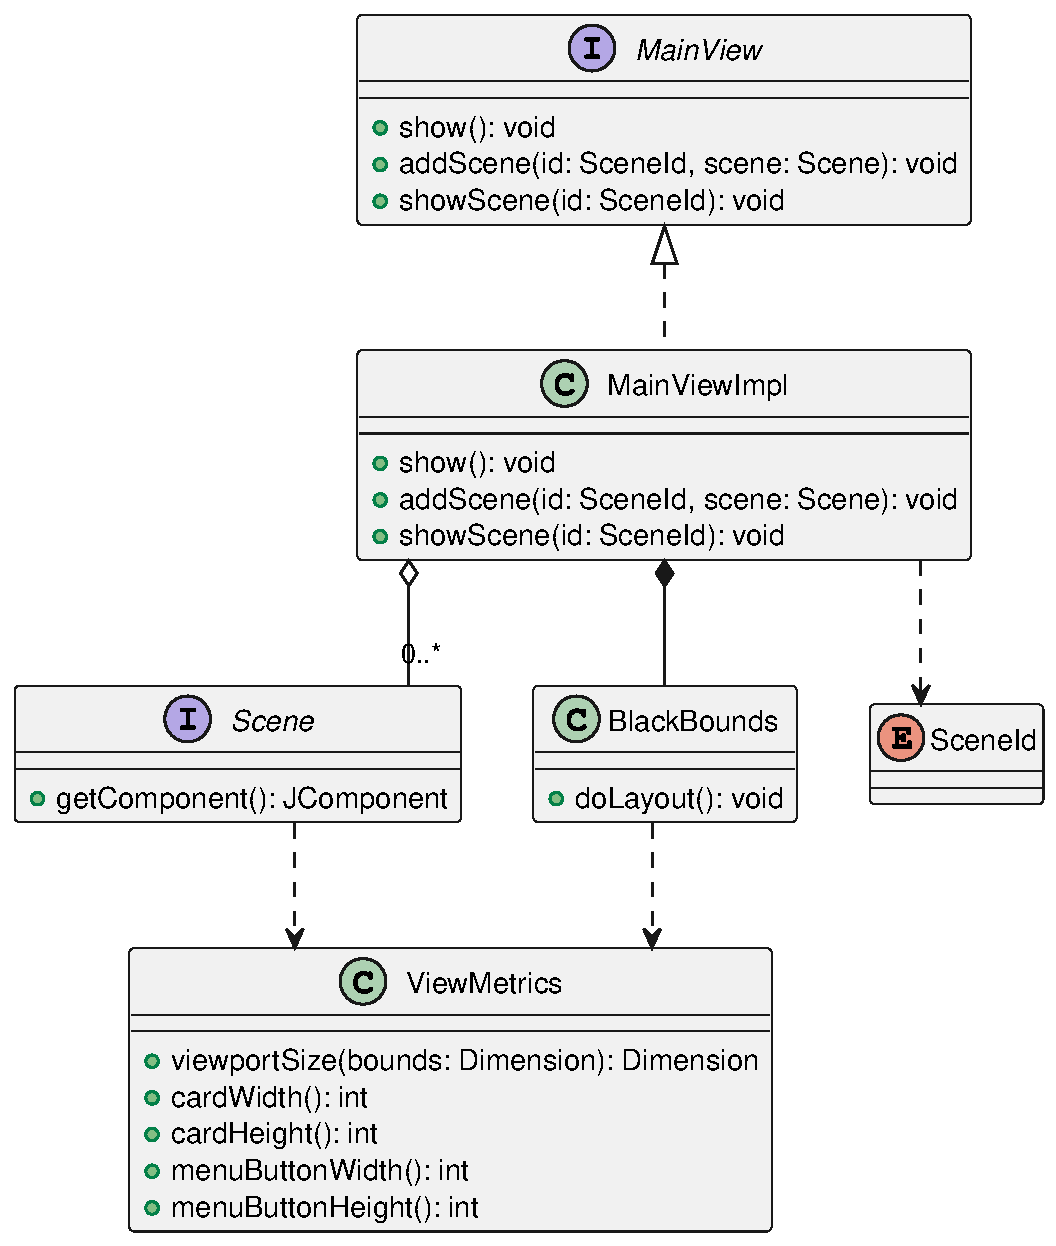
\includegraphics[width=\textwidth]{UMLs/ViewportAdattamento.pdf}
    \caption{Schema UML dell'adattamento della viewport al rapporto 16:9.}
\end{figure}

\subsubsection{Multi-Risoluzione per schermi Hi-DPI}

\textbf{Problema:} Nelle ultime fasi di sviluppo è emerso un bug legato alla
qualità delle immagini delle carte. Il problema non si presentava in modo
uniforme: su alcuni schermi le texture risultavano nitide, mentre su altri
apparivano sgranate o sfocate, senza che inizialmente fosse riconoscibile un
legame evidente con la risoluzione nominale del monitor.

L'analisi successiva ha ricondotto il comportamento agli schermi Hi-DPI. Su
questi dispositivi il sistema operativo può applicare uno \textit{zoom} logico:
l'interfaccia continua a ragionare in pixel logici, ma ogni pixel logico viene
poi rappresentato tramite più pixel fisici. Questa scelta evita che finestre e
componenti diventino troppo piccoli su pannelli molto densi, ma introduce una
differenza tra la dimensione richiesta da Swing e la dimensione realmente usata
dal dispositivo di output. Nel caso specifico, le classi della View ottenevano le
immagini tramite \texttt{ImageLoader}, che le restituiva già scalate alle
dimensioni calcolate da \texttt{ViewMetrics}. Quando però Swing disegnava quelle
icone su uno schermo con fattore di scala maggiore di 1, l'immagine già ridotta
veniva adattata a una superficie fisica più grande, producendo l'effetto di
sgranatura osservato sulle carte.

\textbf{\\Soluzione:} L'idea adottata è stata quella di non trattare più una
richiesta di immagine scalata come una singola bitmap, ma come un'immagine
multi-risoluzione. Per ogni risorsa grafica richiesta a una certa dimensione
logica viene preparata una variante coerente con quella dimensione e, quando
necessario, una seconda variante coerente con la dimensione fisica del
dispositivo. In questo modo le classi della View continuano a chiedere immagini
in termini di pixel logici, ma il sottosistema grafico di Java può selezionare
la variante più adatta al momento del disegno.

Il punto centrale del fix è \texttt{AsyncCachedImageRepository}, che implementa
\texttt{ImageRepository} ed è usata da \texttt{ImageLoaderProxy} dietro alla
facciata statica \texttt{ImageLoader}. Quando riceve una
\texttt{ImageLoadRequest} scalata, il repository calcola prima la dimensione
fisica equivalente tramite il metodo \texttt{deviceSize(int, int)}. Questo metodo
legge il \texttt{defaultTransform} della configurazione grafica principale,
ottenuta da \texttt{GraphicsEnvironment}, e moltiplica larghezza e altezza
logiche per i fattori di scala dello schermo. Nei contesti senza ambiente
grafico viene invece usato un fattore 1.0, così il caricamento resta valido anche
in esecuzioni headless.

Una volta note le due dimensioni, \texttt{AsyncCachedImageRepository} costruisce
l'icona nel metodo \texttt{createScaledIcon}. La risorsa originale viene letta
con \texttt{ImageIO} come \texttt{BufferedImage}, così può essere ridimensionata
in modo controllato. Se dimensione logica e dimensione fisica coincidono, viene
restituita una normale \texttt{ImageIcon}. Se invece lo schermo richiede più
pixel fisici, viene creata una \texttt{BaseMultiResolutionImage} contenente la
variante logica e quella fisica, poi incapsulata in una \texttt{ImageIcon}. Le
chiavi della cache delle immagini scalate includono sia la dimensione logica sia
quella fisica, evitando di riutilizzare per errore la stessa bitmap su schermi
con fattori di scala diversi.

Il ridimensionamento non usa più direttamente \texttt{getScaledInstance}, ma una
procedura esplicita basata su \texttt{Graphics2D}. Il metodo \texttt{scaleImage}
riceve l'immagine sorgente e la dimensione obiettivo, poi la riduce con passi
intermedi: finché la distanza dal risultato finale resta elevata, la bitmap
viene dimezzata; solo alla fine viene prodotta la dimensione esatta. Ogni
passaggio è disegnato da \texttt{renderScaledImage} con interpolazione bicubica,
qualità di rendering elevata e antialiasing. Questa scelta aumenta leggermente
il costo del precaricamento, ma concentra il lavoro in un punto controllato e
produce una qualità più stabile.

Le classi che mostrano effettivamente le carte non devono conoscere il dettaglio
Hi-DPI. \texttt{CardComponent} continua a caricare fronte e retro tramite
\texttt{ImageLoader}. Le misure restano quelle di \texttt{ViewMetrics}; nel
metodo \texttt{paintComponent} il componente disegna l'immagine ricevuta nello
spazio del bottone. Analogamente \texttt{CardsPanel} usa lo stesso caricatore per
costruire gli \texttt{IconPanel} del database. Il catalogo
\texttt{ImagePreloadCatalog} produce invece le richieste scalate per carte,
bottoni e banner, così \texttt{ImageLoader} può precaricare le varianti prima
della visualizzazione delle scene.

Prima di stabilizzare questa soluzione sono stati valutati anche refactor
alternativi. In particolare è stato provato un approccio in cui l'immagine ad
alta risoluzione veniva mantenuta più a lungo e ridimensionata nel punto più
vicino possibile al disegno finale. La qualità visiva era promettente, ma il
compromesso risultava meno adatto all'applicazione: il costo dello scaling
tendeva a spostarsi sul primo rendering dei componenti, oppure rendeva il
precaricamento più pesante e meno prevedibile nelle schermate con molte carte.
La soluzione multi-risoluzione centralizzata nel repository è quindi risultata
più equilibrata, perché mantiene l'API della View invariata, conserva il
precaricamento asincrono già presente e delega a Java la scelta della variante
grafica corretta per lo schermo in uso.

\subsubsection{Stato Simulabile per l'IA}

\textbf{Problema:} L'approccio scelto per l'implementazione dell'IA in fase di
progettazione ha da subito evidenziato un concetto inevitabile: per permettere
all'IA di valutare l'applicazione di determinate mosse sullo stato della
partita, era necessario che queste venissero effettivamente applicate sul tavolo
da gioco, ma modificare direttamente lo stato reale del match avrebbe compromesso
la partita in corso.

\textbf{\\Soluzione:} La soluzione più logica è stata dunque introdurre una
rappresentazione separata dello stato della partita, ricostruita in un contesto
simulato e interamente modificabile. Questo ruolo è affidato all'interfaccia
\texttt{AiGameState} e alla sua implementazione \texttt{AiGameStateImpl}, che
espongono le operazioni minime necessarie alla pianificazione: danneggiare un
giocatore, consumare mana, giocare una carta, danneggiare o rimuovere una carta
dal campo e produrre una copia dello stato corrente.

La costruzione dello stato simulabile è delegata a
\texttt{AiGameStateFactory}, implementata da \texttt{AiGameStateFactoryImpl}.
La factory interroga lo stato reale attraverso \texttt{BoardGame} e costruisce
lo snapshot copiando i dati dello stato reale e usando copie delle carte.
Lo stato del giocatore umano viene creato in maniera dedicata per evitare di
copiare dati sensibili che dal punto di vista dell'IA non sono accessibili.

Le informazioni dei singoli giocatori sono isolate dietro \texttt{PlayerState}
e \texttt{PlayerStateImpl}. Questa classe mantiene l'identificativo del
giocatore, la sua salute, il mana attuale, l'eventuale mano e l'armata in campo, mentre
\texttt{CardStateImpl} rappresenta gli stati delle carte copiate.

Infine l'interfaccia \texttt{AiStateTransition} completa l'implementazione, rappresentando
il concetto di transizione da uno stato simulato a un altro.
La classe \texttt{AiStateTransitionImpl} infatti crea una copia dello stato
ricevuto e poi la modifica in base all'azione da applicare:
\texttt{PlayCardAction} consuma mana e sposta la carta dalla mano all'armata,
\texttt{AttackHeroAction} riduce la salute dell'eroe avversario, mentre
\texttt{AttackCardAction} applica i danni a entrambe le creature e rimuove
quelle sconfitte.
Gli algoritmi decisionali possono così avere un riferimento a questa classe e utilizzarla
per esplorare scenari successivi senza dipendere dalle regole concrete di modifica dello stato.

\begin{figure}[htbp]
    \centering
    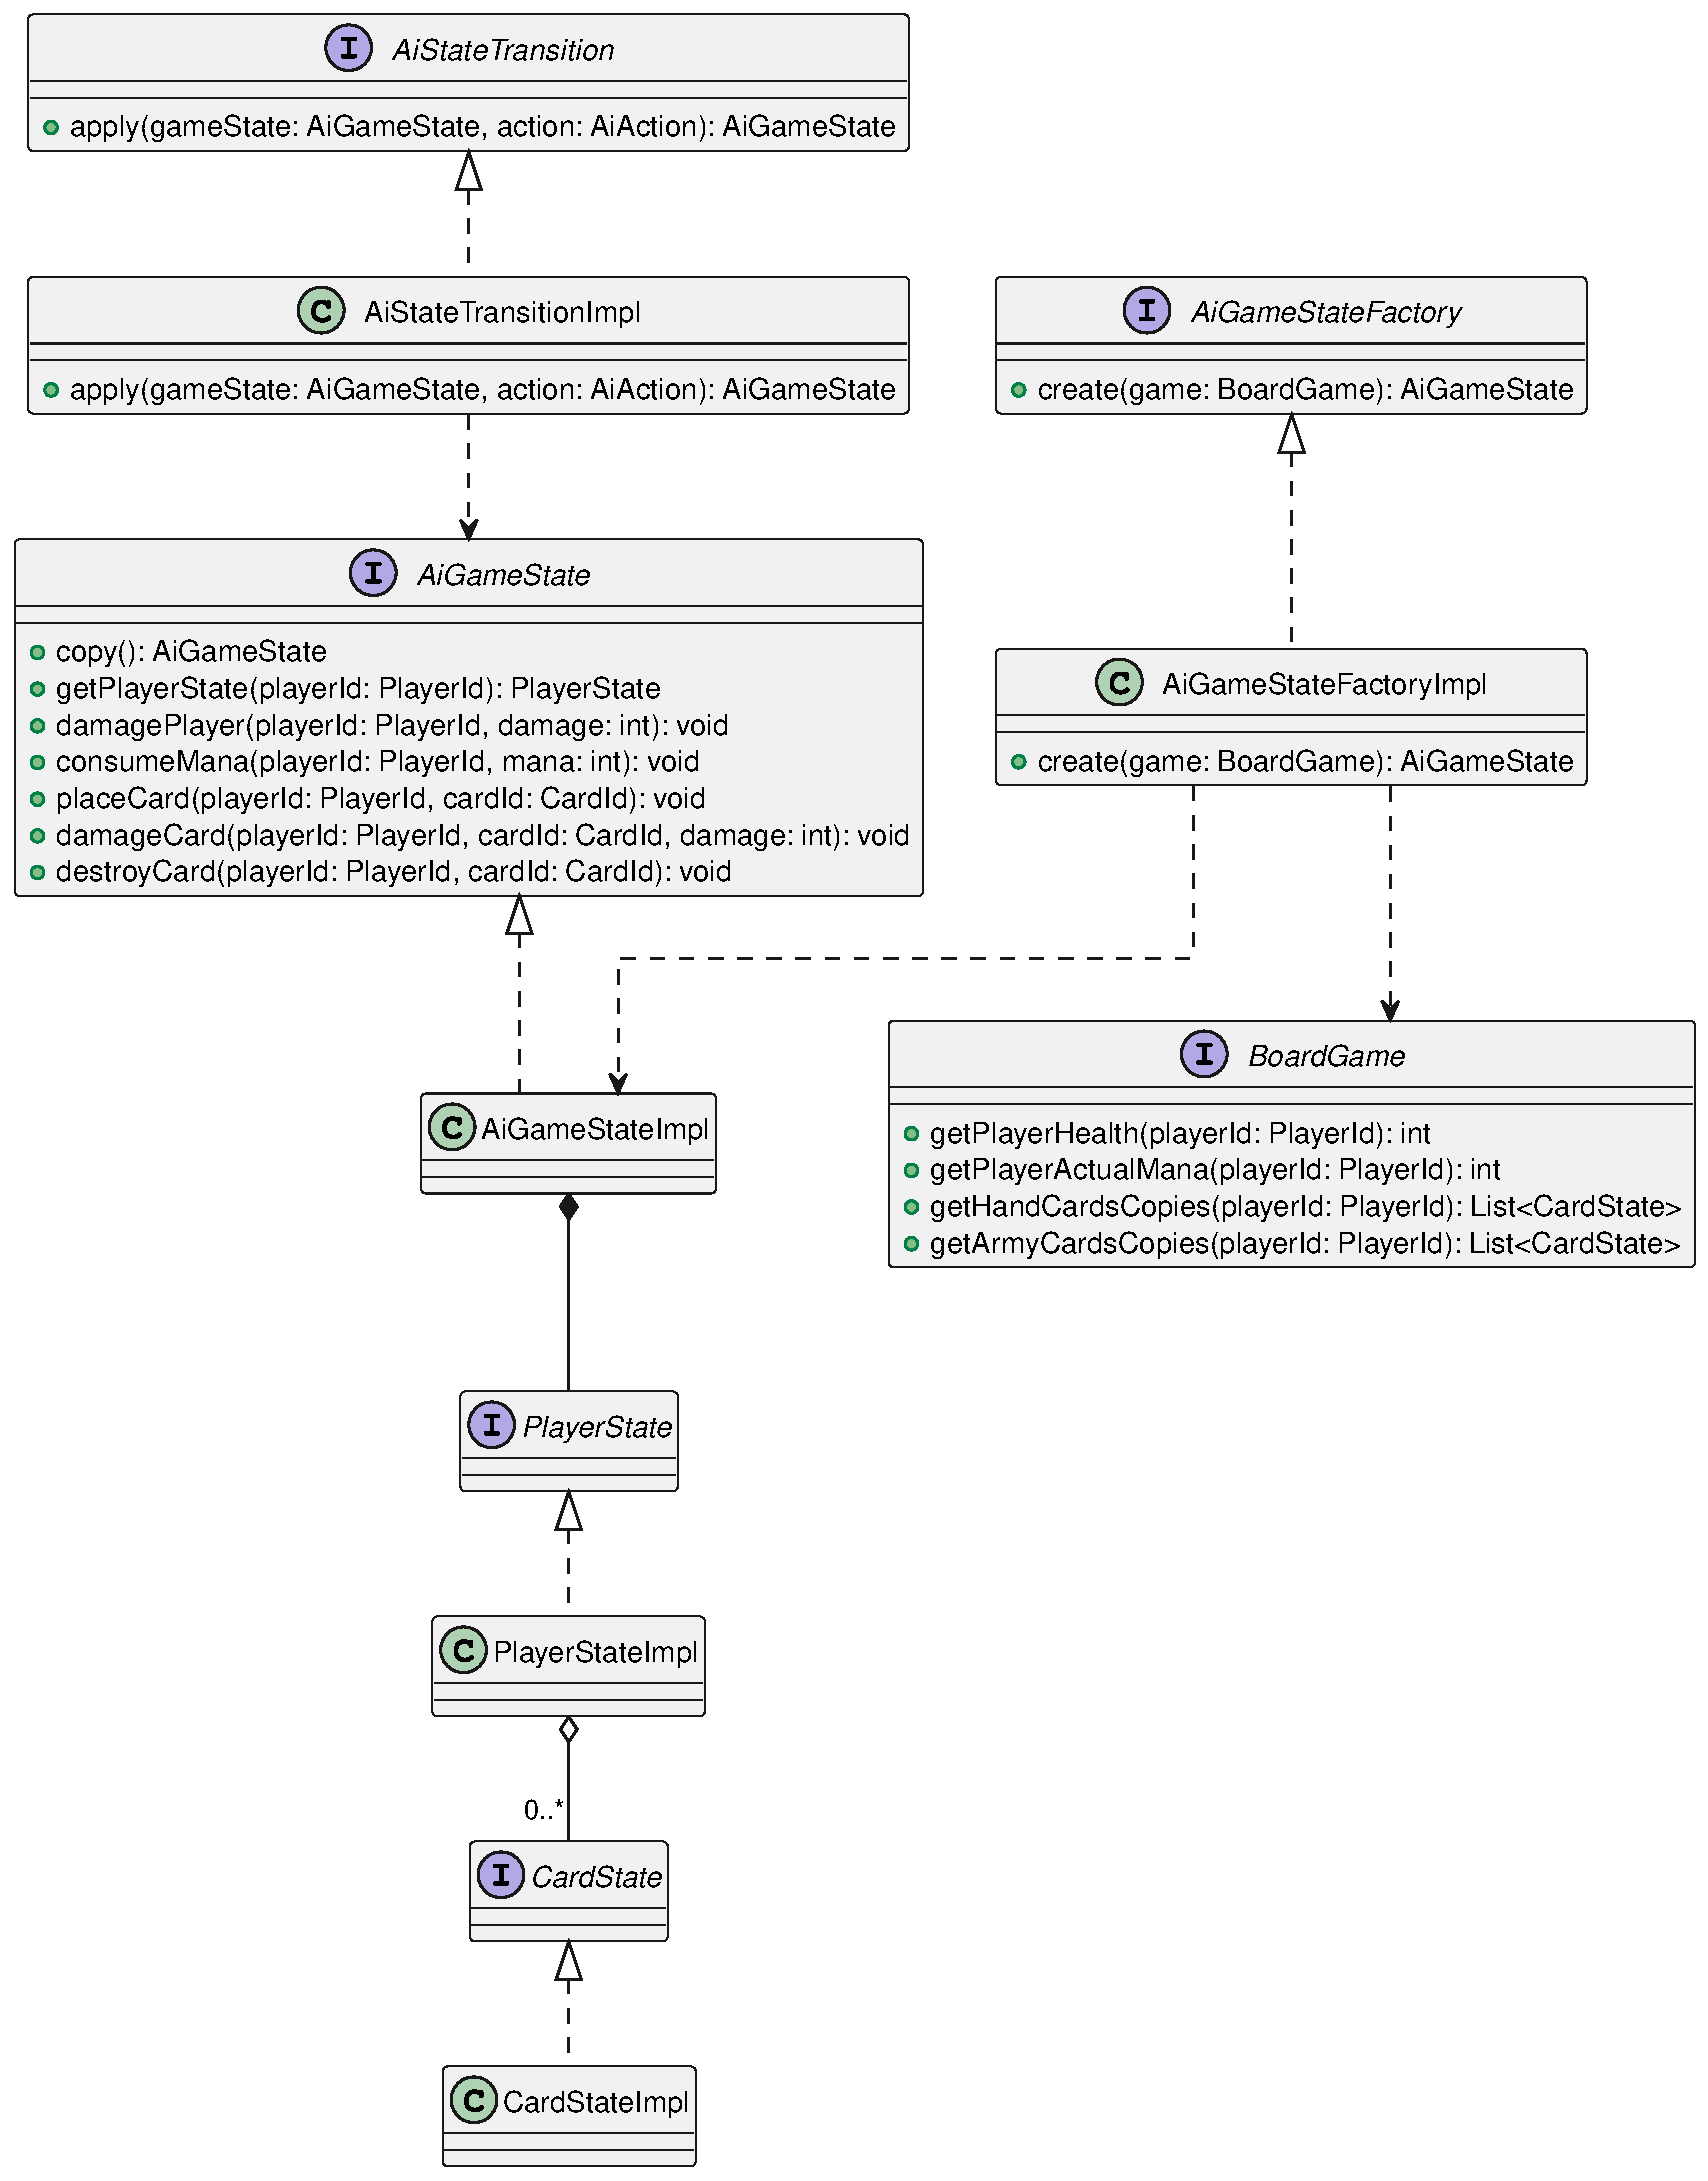
\includegraphics[width=\textwidth]{UMLs/AiStatoSimulabile.pdf}
    \caption{Schema UML dello stato simulabile utilizzato dall'intelligenza artificiale.}
\end{figure}

\subsubsection{Politica Decisionale Sostituibile per l'IA}

\textbf{Problema:} A un certo punto dell'implementazione dell'IA, è sorta la necessità
di integrarla con il ciclo reale del turno. L'algoritmo poteva
scegliere una sequenza di mosse su uno stato astratto, ma tali decisioni dovevano
poi essere applicate alla partita effettivamente giocata dall'utente. Inoltre la
selezione della difficoltà richiedeva di poter sostituire la politica
decisionale senza modificare il controller della partita o le regole del modello.

\textbf{\\Soluzione:} La soluzione adottata separa la scelta delle mosse dalla
loro esecuzione reale. Il punto di raccordo principale è rappresentato
dall'interfaccia \texttt{AiTurnService} e dalla classe \texttt{AiTurnServiceImpl}.
Il servizio riceve il \texttt{BoardGame} corrente, usa
\texttt{AiGameStateFactory} per costruire lo snapshot simulabile e delega la
decisione a un oggetto di tipo \texttt{AiDecisionAlgorithm}. Il controller della
partita non deve quindi conoscere il funzionamento interno dell'IA: richiede
soltanto il piano del turno e ottiene una lista ordinata di \texttt{AiAction}.

La sostituibilità della politica decisionale è ottenuta applicando il pattern
\textit{Strategy}. L'interfaccia \texttt{AiDecisionAlgorithm} definisce il
contratto comune degli algoritmi, mentre le implementazioni
\texttt{GreedySequentialAiAlgorithm} e
\texttt{DepthLimitedLookaheadAiAlgorithm} rappresentano due strategie
alternative. La prima sceglie iterativamente la migliore azione che produce un
miglioramento immediato dello stato, la seconda esplora sequenze di azioni fino
a una profondità limitata e seleziona quella con la valutazione euristica
migliore. Entrambe usano gli stessi componenti di supporto:
\texttt{AiActionGeneratorImpl} per generare le azioni legali,
\texttt{AiStateTransitionImpl} per applicarle allo stato simulato e
\texttt{HeuristicAiStateEvaluator} per assegnare un punteggio agli scenari.

La scelta concreta della strategia avviene in \texttt{MainControllerImpl}, dove
una mappa associa \texttt{Difficulty.NORMAL} a
\texttt{GreedySequentialAiAlgorithm} e \texttt{Difficulty.HARD} a
\texttt{DepthLimitedLookaheadAiAlgorithm}. Quando l'utente avvia una partita,
il controller costruisce \texttt{AiTurnServiceImpl} passando l'algoritmo
corrispondente alla difficoltà selezionata. In questo modo l'aggiunta di una
nuova difficoltà o di un nuovo algoritmo richiede soltanto una nuova
implementazione della strategia e la sua registrazione nel punto di creazione.

L'applicazione delle azioni decise dall'IA è invece responsabilità di
\texttt{AiActionExecutor}, implementata da \texttt{AiActionExecutorImpl}. Questa
classe traduce le azioni astratte prodotte dagli algoritmi nelle operazioni
effettive di \texttt{BoardGame}: posizionare una carta, attaccare l'eroe
avversario oppure attaccare una creatura. Per farlo invoca rispettivamente
\texttt{place}, \texttt{attackHero} e \texttt{attackCard}. Il
\texttt{MatchController} rimane così il coordinatore del turno, ma non
contiene logica decisionale né dettagli di conversione tra azioni simulate e
azioni reali.

\begin{figure}[htbp]
    \centering
    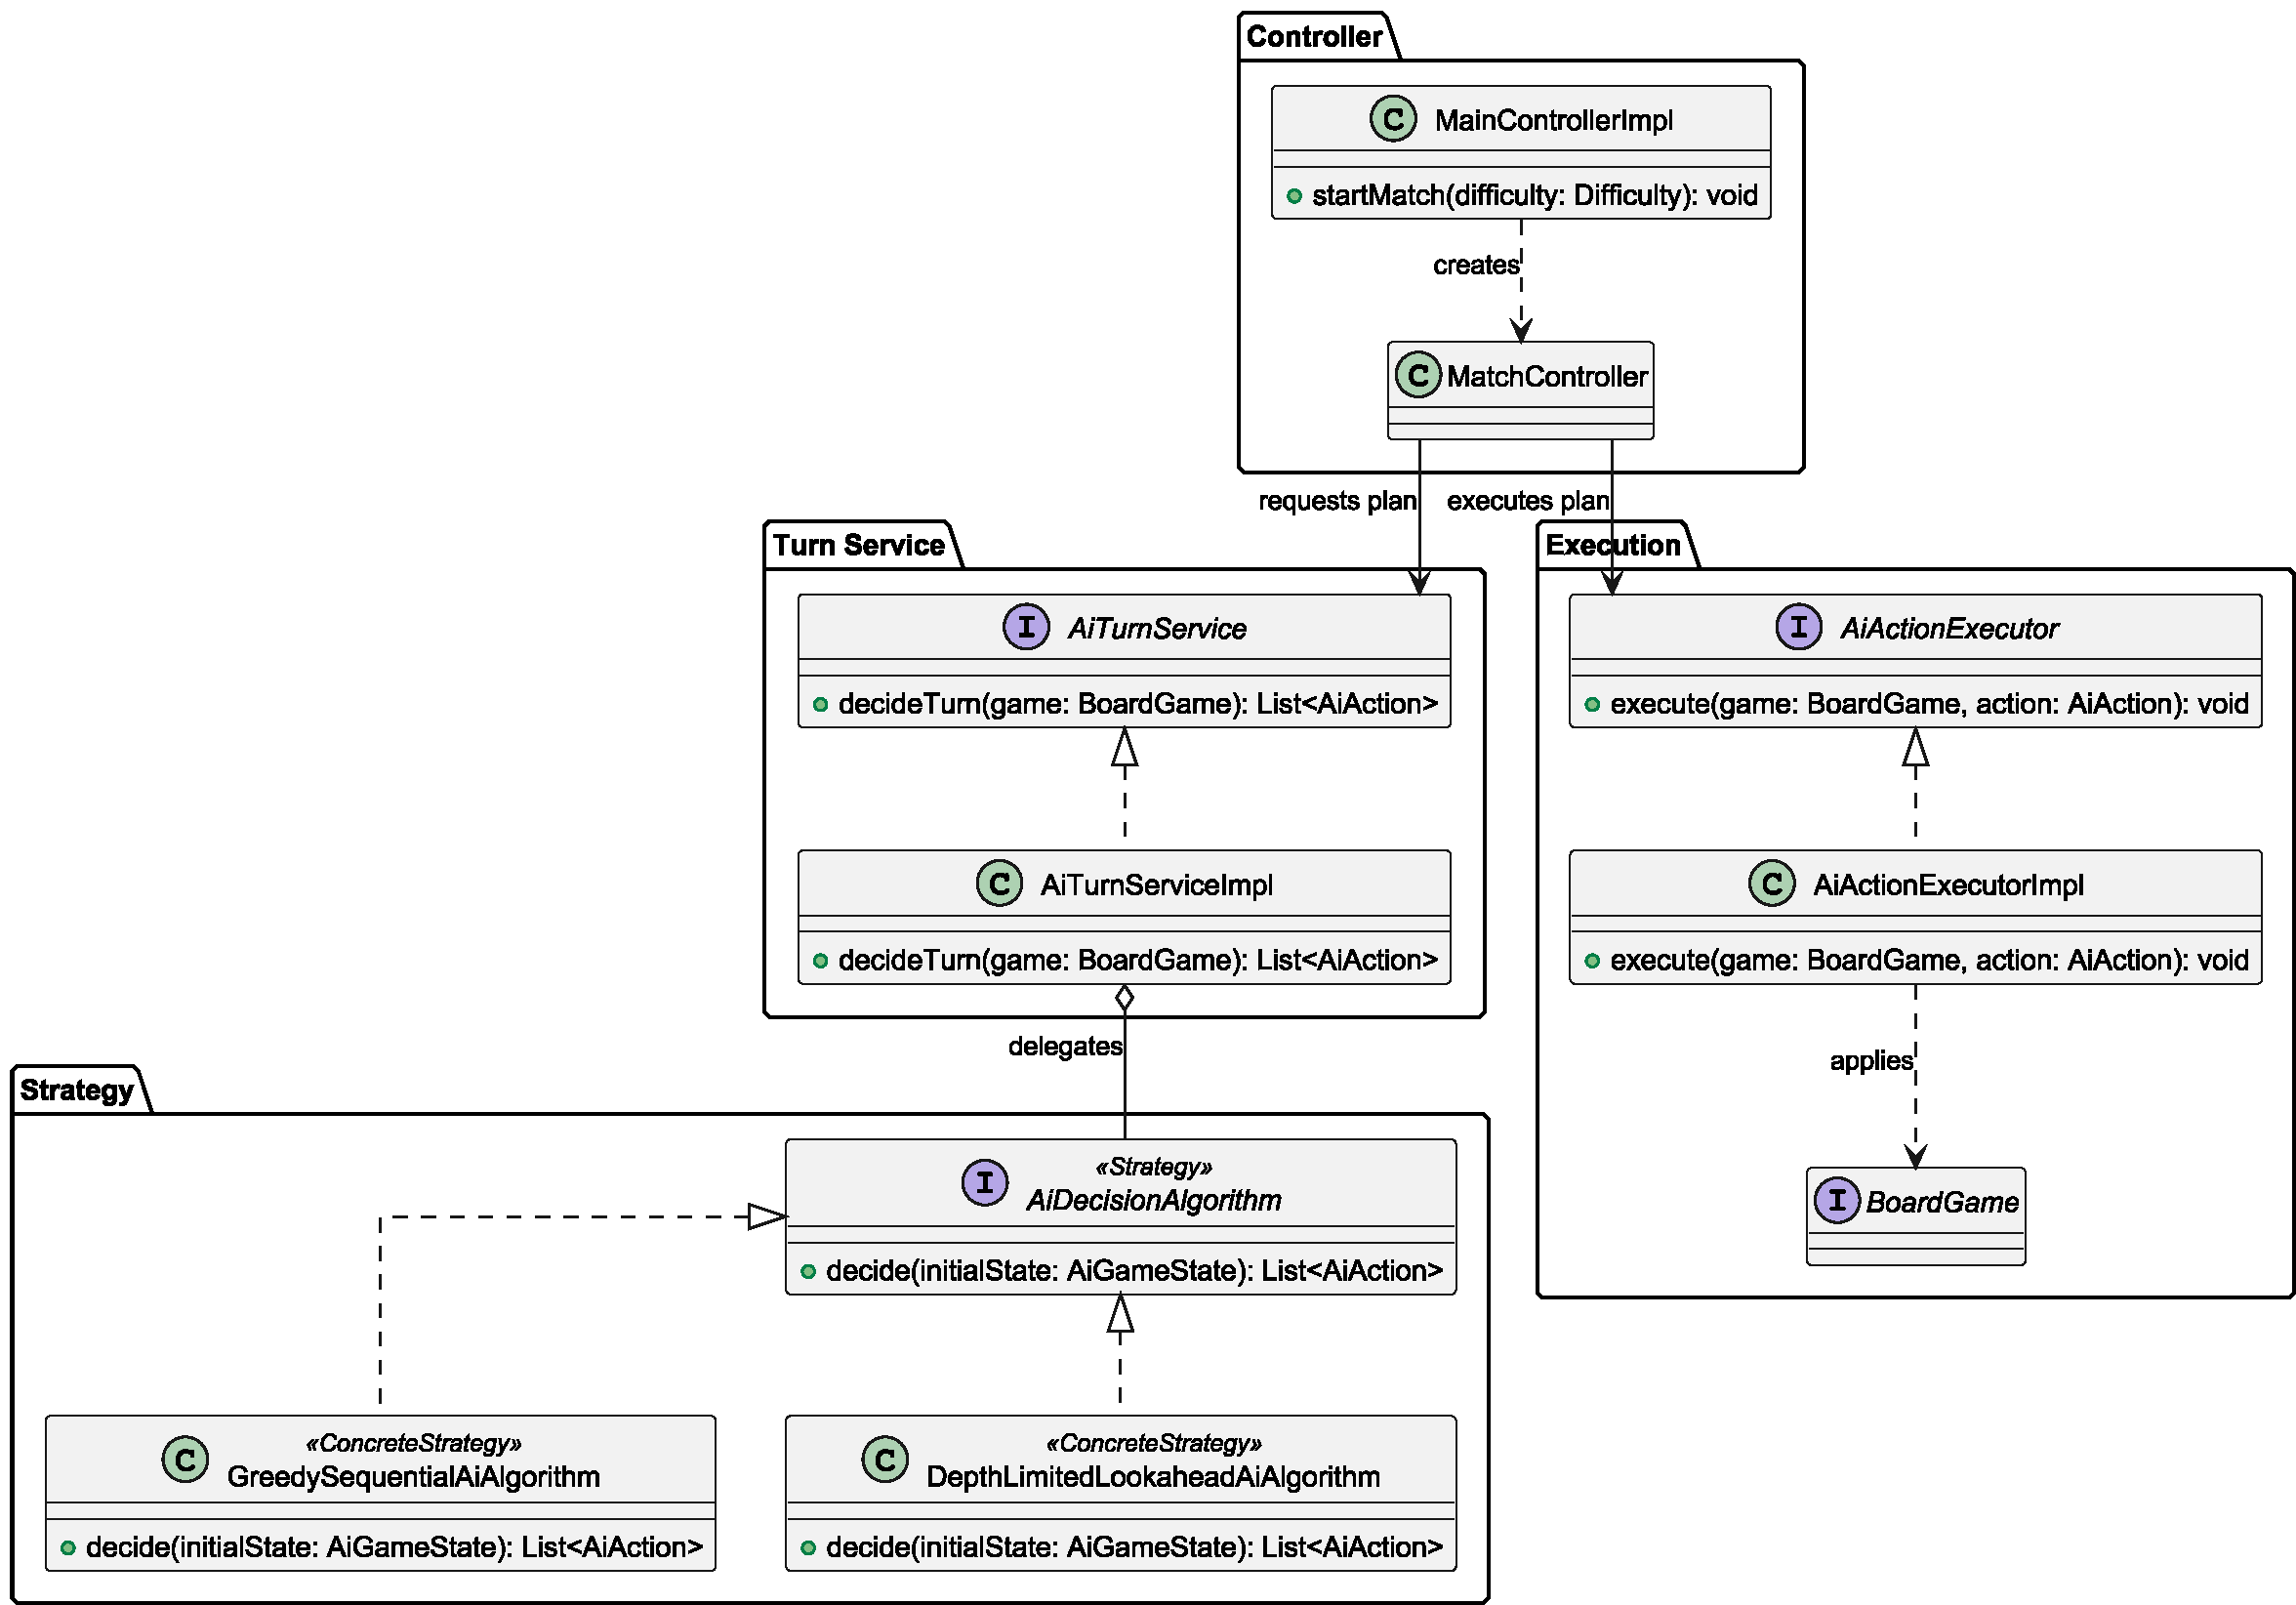
\includegraphics[width=\textwidth]{UMLs/AiPoliticaDecisionale.pdf}
    \caption{Schema UML della politica decisionale sostituibile dell'intelligenza artificiale.}
\end{figure}
